\documentclass[10pt,letterpaper]{article}
\usepackage{geometry}
\usepackage{float}
\geometry{margin=1in}
\usepackage{graphicx}

\usepackage{booktabs}
\usepackage{amsmath}

\setlength{\parindent}{0pt}
\setlength{\parskip}{0.5em}

%make lists tighter
\usepackage{enumitem}
\setlist{nolistsep}

%reduce spacing before and after section
\usepackage{titlesec}
% reduce section, subsection, etc spacing
\usepackage{titlesec}
\titlespacing*{\section}{0pt}{0\baselineskip}{0\baselineskip}
\titlespacing*{\subsection}{0pt}{0\baselineskip}{0\baselineskip}
\titlespacing*{\subsubsection}{0pt}{0\baselineskip}{0\baselineskip}

%reduce list spacing
\usepackage{enumitem}
\setlist{nosep}

\usepackage[hidelinks]{hyperref}

\title{Final Project, Stat 215A, Fall 2024\vspace{-2em}}

% submission must not contain any of your names
% but feel free to make a version for yourself with your names on it
% \author{Your names}

\begin{document}
\maketitle

\section{Introduction}

Cervical spine injuries (CSI) resulting from blunt trauma to the neck and upper back, including the posterior head region, pose a significant threat to patients. Initial management often involves immobilization to prevent further injury during transportation to the hospital or emergency department (ED). However, recent studies have raised concerns that cervical spine immobilization may have detrimental effects on patients, impacting both physical and mental well-being \cite{ham2014pressure, abram2010routine, ottosen2019patient}.

Notably, these studies have primarily focused on adult populations, leaving a knowledge gap regarding the potential consequences of these clinical decision rules on pediatric patients under 16 years old. Pediatric CSI can be particularly devastating, with mortality rates highlighting the need for effective diagnosis and treatment. Additionally, the pediatric CSI represent less than 10\% of the total injuries in a clinical diagnosis data \cite{brown2001cervical}, however, the challenges of diagnosing CSI in children, including their inability to communicate symptoms and tendency to move in restrained positions, further complicate management.

This project aims to address these challenges by leveraging data-driven clinical decision-making. Using the Predicting Cervical Spine Injury in Children dataset from the Pediatric Emergency Care Applied Research Network (PECARN), which comprises data from over 3,000 pediatric patients across 17 hospitals, we seek to improve our understanding of pediatric CSI and inform evidence-based treatment strategies. The clinical decision rule aimed to respond is to understand in a patient, given certain features, requires a cervical immobilization, before or during the medical examination.

Specifically, this study will develop and compare two predictive models – Machine Learning-based and Neural Network-based – with the baseline model proposed by Leonard et al. \cite{leonard2011factors}. We will evaluate the performance of these models using various metrics relevant to the domain problem. Additionally, we will conduct perturbation analysis and feature importance assessments to elucidate the impact of individual variables on the models' predictions. Finally, we will apply our approach to real-case scenarios and discuss the potential benefits and limitations of integrating our models into clinical practice.

\section{Data}
The present data has different datasets mentioned below:
\begin{enumerate}
    \item Information of the patients based on the location of their examination, e.g. on site, offsite, on field.
    \item Demographics of the patients, e.g. age, height
    \item Injury classification of different Cervical Spines Injuries and the description of the mechanism.
    \item Information about the complaints delivered by the patients
    \item Medical history and radiology information of each patient and case.
\end{enumerate}

It is important to discuss that most of the data is Categorical (Binary. True or False) while certain aspects of the data such as Glasgow Coma Scale (GCS) scores are Numerical. As well, there were many columns in string format describing specific cases treatment or characteristics, which might help to understand their diagnosis. In the following section, several aspects of the data is explored, as well trying to understood the main implication of the CSI with the characteristics of each patient's case.

\subsection{Case studies}

Cervical Spine Injuries (CSIs) can be categorized into various types based on their impact on the body, ranging from traumatic fractures to ligamentous failures. The PECARN dataset provides a comprehensive classification of injuries in the \textit{injuryclassification.csv} file, which documents the specific injury type for each case. Figure \ref{fig:injury-site} illustrates the distribution of injury classifications based on the dataset. Notably, all classified injuries are still categorized as CSIs. Therefore, for the purposes of this analysis, we consolidated these injuries into a single summary column, which indicates whether a patient was diagnosed with any type of CSI. Then, we observed how many patients were actually immobilized based on the presence of diagnose of CSI and computed the correct immobilization column. 

\begin{figure}[H]
    \centering
    \begin{minipage}{0.45\textwidth}
        \centering
        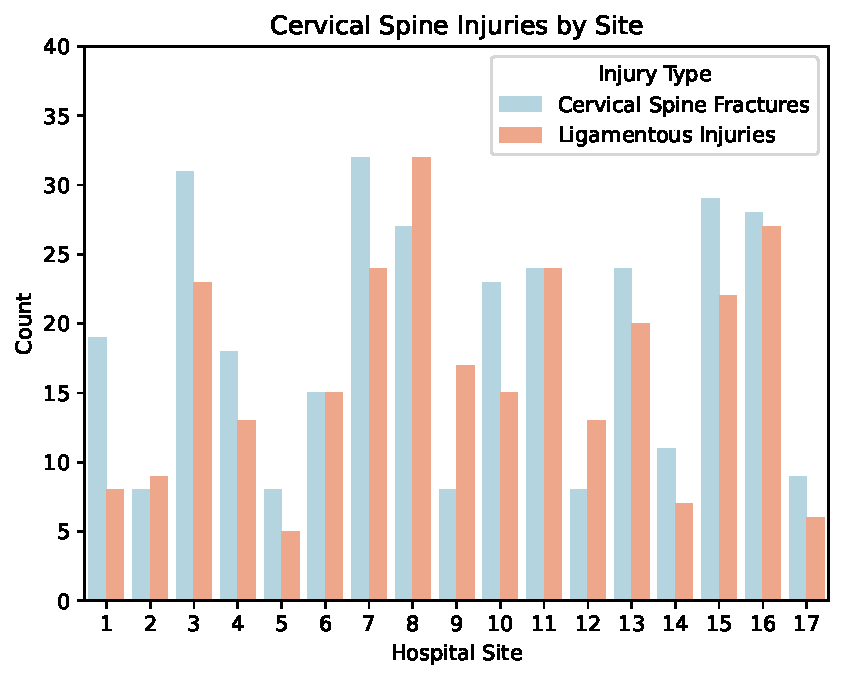
\includegraphics[width=\linewidth]{plots/cervical_spine_injuries_by_site.pdf}
        \caption{Injury classification on each hospital site}
        \label{fig:injury-site}
    \end{minipage}\hfill
    \begin{minipage}{0.45\textwidth}
        \centering
        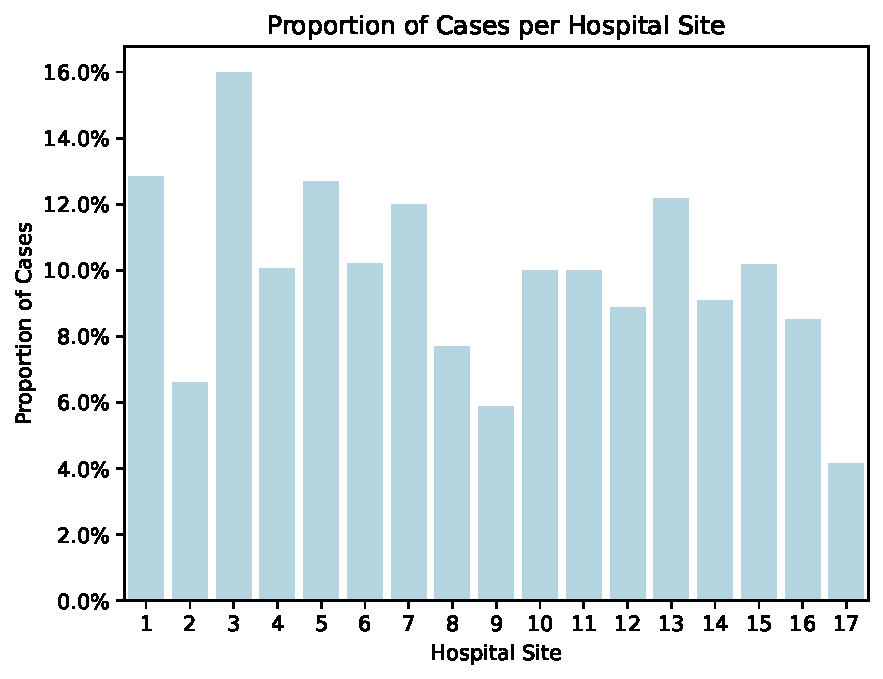
\includegraphics[width=\linewidth]{plots/cases_per_site.pdf}
        \caption{Proportion of cases present on each hospital site}
        \label{fig:cases-site}
    \end{minipage}
\end{figure}

\subsection{Findings}
Usually the Glascow Coma Scale (GCS) is refered as a measure of how conscious is the patient at the time of the evaluation. According to the Canadian C-spine rule \cite{stiell2001canadian} also referes to the score parameter as a decision rule for immobilization of patients. However, as shown in Figure \ref{fig:gcs-target} , actually the amount of people below the concious value (e.g. 15) is below the amount of people with good GCS.

\begin{figure}[H]
    \centering
    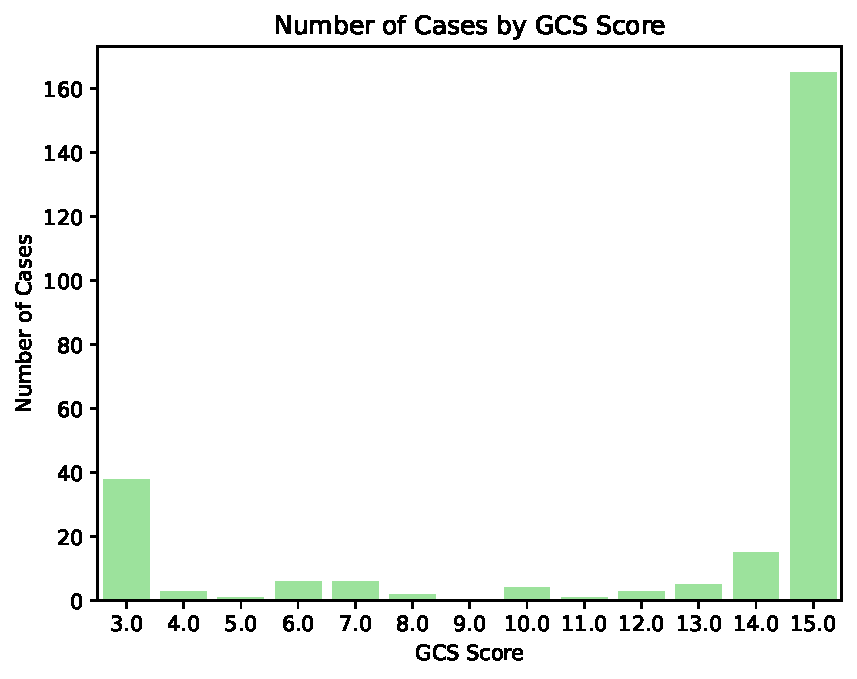
\includegraphics[width=0.5\linewidth]{plots/cases_by_gcs.pdf}
    \caption{Number of correct immobilization by each GCS}
    \label{fig:gcs-target}
\end{figure}

The figure fits with the critique that decision rules have been taking place on the practitioners \cite{michaleff2012accuracy}. 


\subsection{Data Cleaning}

A quick overview of the characteristics of the data shows that:
\begin{itemize}
    \item Most of the data is represented by binary information, e.g. True and False. 
    \item Float information, as Glasgow Comma Score (GCS) are less frequent. 
    \item All data have been collected by referencing a unique Patient ID information.
\end{itemize}

We've been debating on different ways to deal with all different issues with the dataset. Given that the dataset has a handful of columns(features) and performing a closer investigation needs very specific domain knowledge, we've figured out some uniform ways to deal with some systematic issues, like missing values or misaligned data types. As for inconsistency, we've performed a brief scan on each columns along with their feature description, and figures out whether the entries in each column is actually making sense.

The actual cleaning process is relatively straightforward: We first combine all the information indexing on site, caseid, controltype and Study Subject ID. The rest of the procedure could be summarized as follow:

\begin{enumerate}
    \item Understand if any variable can be comprised into a single column, e.g. the total GCS score rather than the detailed scores for each of the components. 
    \item Understanding the meaning and gathering of information of a column, e.g. Text description of particular patients can be challenging to clean, therefore, \textbf{a judgment call} is to believe the boolean information can be sufficient.
    \item some columns includes additional text input to describe some special circumstances. We've converted those columns into a single binary column, which indicates whether additional text information is being provided.
    \item Any mis-aligned datatype have been corrected, only having the types of floats, integers, and booleans.
    \item Any feature with missing values is filled with -1, as an encoding of missing in data. 
    \item Any unspecified data entries (for instance, an 'NP' or 'S' in a binary or numerical columns) are all converted to -1. 
    \item We've finally dropped any time/datetime entries, as heuristically our model should be date/time agnostic.
\end{enumerate}

\section{Modeling and Evaluation}

\subsection{Metric}

Accurate diagnosis of cervical spine injuries (CSI) in children is crucial, as false diagnoses can have severe consequences, including immobilization-related injuries and unnecessary radiation exposure from CT scans \cite{brown2001cervical}. To minimize false positives and false negatives, our group selected the F1-score as the primary evaluation metric, which is defined mathematically as:

\begin{equation}
    F1 = 2 \times \frac{Precision \times Recall}{Precision + Recall}
\end{equation}

The F1-score effectively balances precision and recall, considering both false positives and false negatives simultaneously. Its flexibility makes it well-suited for handling imbalanced datasets. F1 score performs slightly better than other metrics in medical diagnoses when prevalence is low, which makes it perfect for our dataset since there's a huge data imbalance \cite{hicks2022evaluation}.

While the F1 score is our primary metric, we acknowledge that no single metric fully captures a model's goodness-of-classification \cite{hicks2022evaluation}. Therefore, we consider additional metrics, graphs, and probabilities to ensure a holistic evaluation of our models. This comprehensive approach provides a more nuanced understanding of our models' performance and enables informed decision-making.

\subsection{Data splitting and resampling}

The dataset, comprising diagnoses from multiple patients across different locations and time points, prompted us to consider the optimal granularity for analysis. Notably, the Site, SubjectID, and CaseID columns were consistently present across all data points, without requiring additional cleaning or preprocessing. Among these columns, the Site variable captured spatial information, categorizing patients into distinct emergency department (ED) locations. Different sites have inherent bias injected upon while during the data collection process, resulting in a ditributional shift in the data. Thus making sure site information is randomized across the training and validation set is crucial. This is further discussed in the stabiltiy test section, which we analyzed the feasibility of our model generalizing across different sites.

The implementation of the data splitting was mostly text-book style train test split with scikit-learn. While training the model, we've also used K-Fold cross validation to make sure the model is not overfitting on the training data and our model is using the best set of hyperparameters.

The purpose for resampling the data is to make sure the model is not biased towards the majority class. Aparently 90\% of the cases are Negative, making it hard for the model to generalize on the minority class. We've used SMOTE to oversample the minority class, creating a balance between the two classes.

\subsection{Baseline model}
The original paper \cite{leonard2011factors} developed certain analysis variables based on domain knowledge and data inference, which is contained in the following table:

\begin{table}[H]
\centering
\begin{tabular}{cc}
\textbf{Description}              & \textbf{Variable}                                             \\ \hline
Altered mental status             & GCS                                                           \\
Loss of consciousness             & Based on qualitative metrics                                                              \\
Non ambulatory                    & If the patient can move freely                                                              \\
Focal neurologic findings        &  Based on any focal injury symptoms                                                             \\
Complaint of neck pain            &  Description of neck pain from the patient                                                             \\
Posterior midline neck tenderness &  Based on the rotation and movement of the midline neck                                                             \\
Any neck tenderness               & Any documented tenderness on physical examination of the neck \\
Torticollis                       & Limited range of motion                                       \\
Substantial injury                & Life threatening injuries                                     \\
High risk mechanism               & Injury mechanism categorized as High Risk                     \\ \hline
\end{tabular}
\caption{Analysis variables used in the original study \cite{leonard2011factors}}
\label{tab:base_variables}
\end{table}

The following variables there were fitted in a Random Forest (RF) algorithm to classify the presence of any CSI in the patient. 

\begin{table}[H]
\centering
\footnotesize
\begin{tabular}{lllll}
\toprule
\textbf{Specificity} & \textbf{Sensitivity} & \textbf{Recall} &  \textbf{F1-Score}\\
0.0926 & 0.937  & 0.105 & 0.1895  \\
\bottomrule
\end{tabular}
\caption{Performance of RF Baseline model on testing set}%
\label{tab:svm_results}
\end{table}

Replicating this approach with our random forest model with a threshold that ensures at least 90\% sensitivity while maximizing the F1-score on the validation set, we were able to achieve a sensitivity of approximately 93.75\% on the test set, with a specificity of about 9.26\%, a precision of around 10.54\%, an F1-score of roughly 18.95\%, and lastly a false negative rate of about 6.25\%.

\begin{figure}[H]
    \centering
    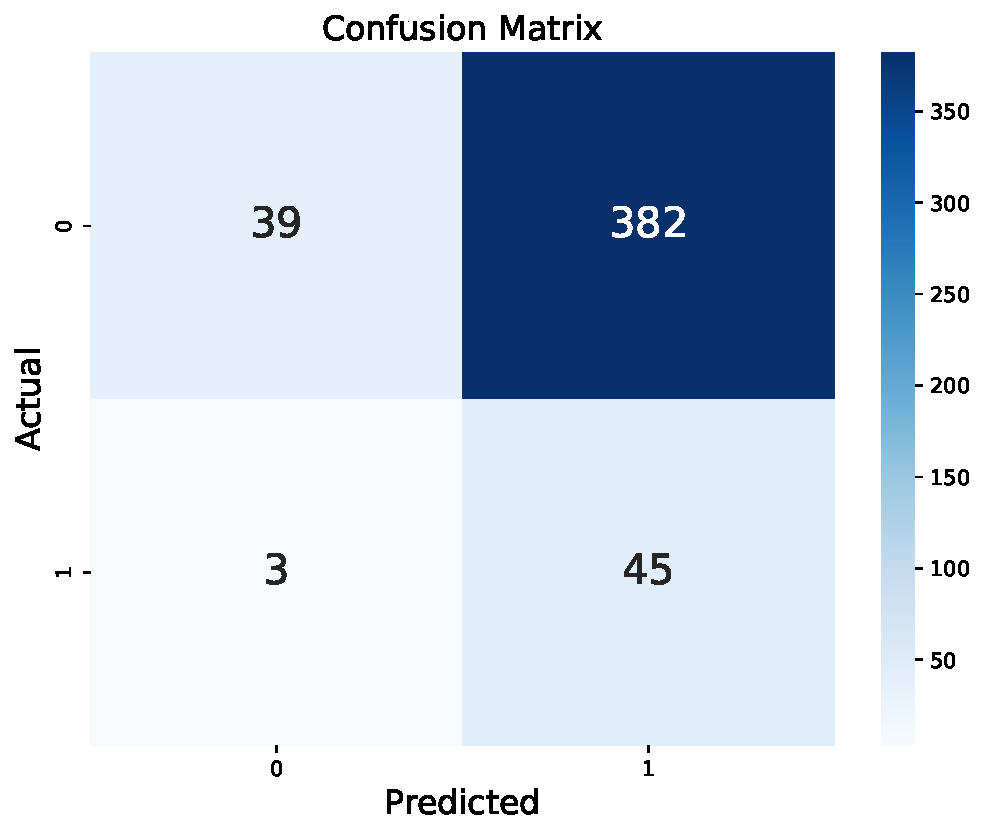
\includegraphics[width=0.5\linewidth]{plots/confusion_matrix_baseline.pdf}
    \caption{Baseline Confusion Matrix}
    \label{fig:confusion-baseline}
\end{figure}

Additionally, as observed on Figure \ref{fig:confusion-baseline}, the high ratio of False Negative (FN) represent a tread in the determination of the model as a medical decision rule, since this would imply that the best choice is to always immobilize the patient. 

\subsection{SVM}
In addition to the baseline model and dimensionality reduction methods described above, we also trained on Support Vector Machine (SVMs) model as a supervised learning method. SVM is a supervised machine learning algorithm used often in classification of binary outcomes ~\cite{svm}. In this study, SVM was used to predict cervical spine fractures, which achieved lowest False Negative counts on validation set. The dataset suffered from high sparsity as the data contained many non-documented values. In addition, categorical values were one-hot encoded, further increasing the sparsity of the dataset. To combat this, SVM was used. SVMs generally perform well on sparse and unbalanced data (if using weighted SVM). To introduce more robustness to the model, we also analyzed class-weighted SVM to deal with unbalanced data by assigning higher misclassification penalties to training instances of the minority class.

First, to accommodate the non-linearity in the dataset, the SVM utilized the radial basis function (RBF) kernel, which maps the input features into a higher-dimensional space, allowing the algorithm to identify complex patterns. Then, we trained on simple SVM model and class-weighted SVM. Both hyperparameters were finetuned using GridSearchCV on validation set using hyperparameter spaces defined in Table~\ref{tab:hyperparams}. As a result, we set a regularizing parameter $C$ as 100, a gamma parameter as 0.01 and used RBF kernel for the model. We, then, evaluated on validation set using these configurations. The results are shown in Table~\ref{tab:svm_results}.

\begin{table}[h!]
\centering
\footnotesize
\begin{tabular}{lllll}
\toprule
\textbf{Hyperparams} & \multicolumn{2}{c}{\textbf{Choices}} \\
\midrule
C (Regularization) & 0.1 & 1 & 10 & 100  \\
Gamma & \text{scale} & 0.01 & 0.1 & 1 \\
Kernel & \text{RBF} & \text{Poly} & \text{Sigmoid}\\
\bottomrule
\end{tabular}
\caption{Hyperparameter choices for SVM}%
\label{tab:hyperparams}
\end{table}

\begin{table}[h!]
\centering
\footnotesize
\begin{tabular}{lllll}
\toprule
\textbf{Model} & \textbf{Accuracy} & \textbf{Precision} & \textbf{Recall} &  \textbf{F1-Score}\\
\midrule
SVM (RBF Kernel) & 0.50 & 0.81  & 0.90 & 0.85  \\
Class-Weighted SVM & 0.51 & 0.81  & 0.89 & 0.85 \\
\bottomrule
\end{tabular}
\caption{Performance of SVM model on validation set}%
\label{tab:svm_results}
\end{table}

Additionally, we analyzed the decision boundary of the best performing model to further study the behavior of its prediction. Figure~\ref{fig:svm_decision} shows the decision boundary plot of the SVM. To interpret this plot, if a red point lies in the blue region, it indicates that a true "Not immobilized" sample was incorrectly classified as "immobilized" - a False Positive. Similarly, if a blue point lies in the red region, it indicates that a true "immobilized" sample was incorrectly classified as "Not immobilized" - a False Negative. In this study, we claim that False Negative is far worse than a False Positive. To align with this, we specifically tested the models' ability to avoid False Negatives. In other words, model's ability to achieve a high specificity (or recall). Figure~\ref{fig:svm_decision} shows that our SVM model correctly classifies points far from the boundary region with high confidence. The majority of both right upper and lower corner clusters are blue points, meaning that decision boundary is well-calibrated. Clusters that are in proximity to the boundary region includes a mix of blue and red points, indicating a model's lack of confidence in the classification for those regions. As a result, while the SVM model performs reasonably well overall, its ability to accurately classify data in highly clustered regions is limited.

\begin{figure}[tb!]
%
\centering
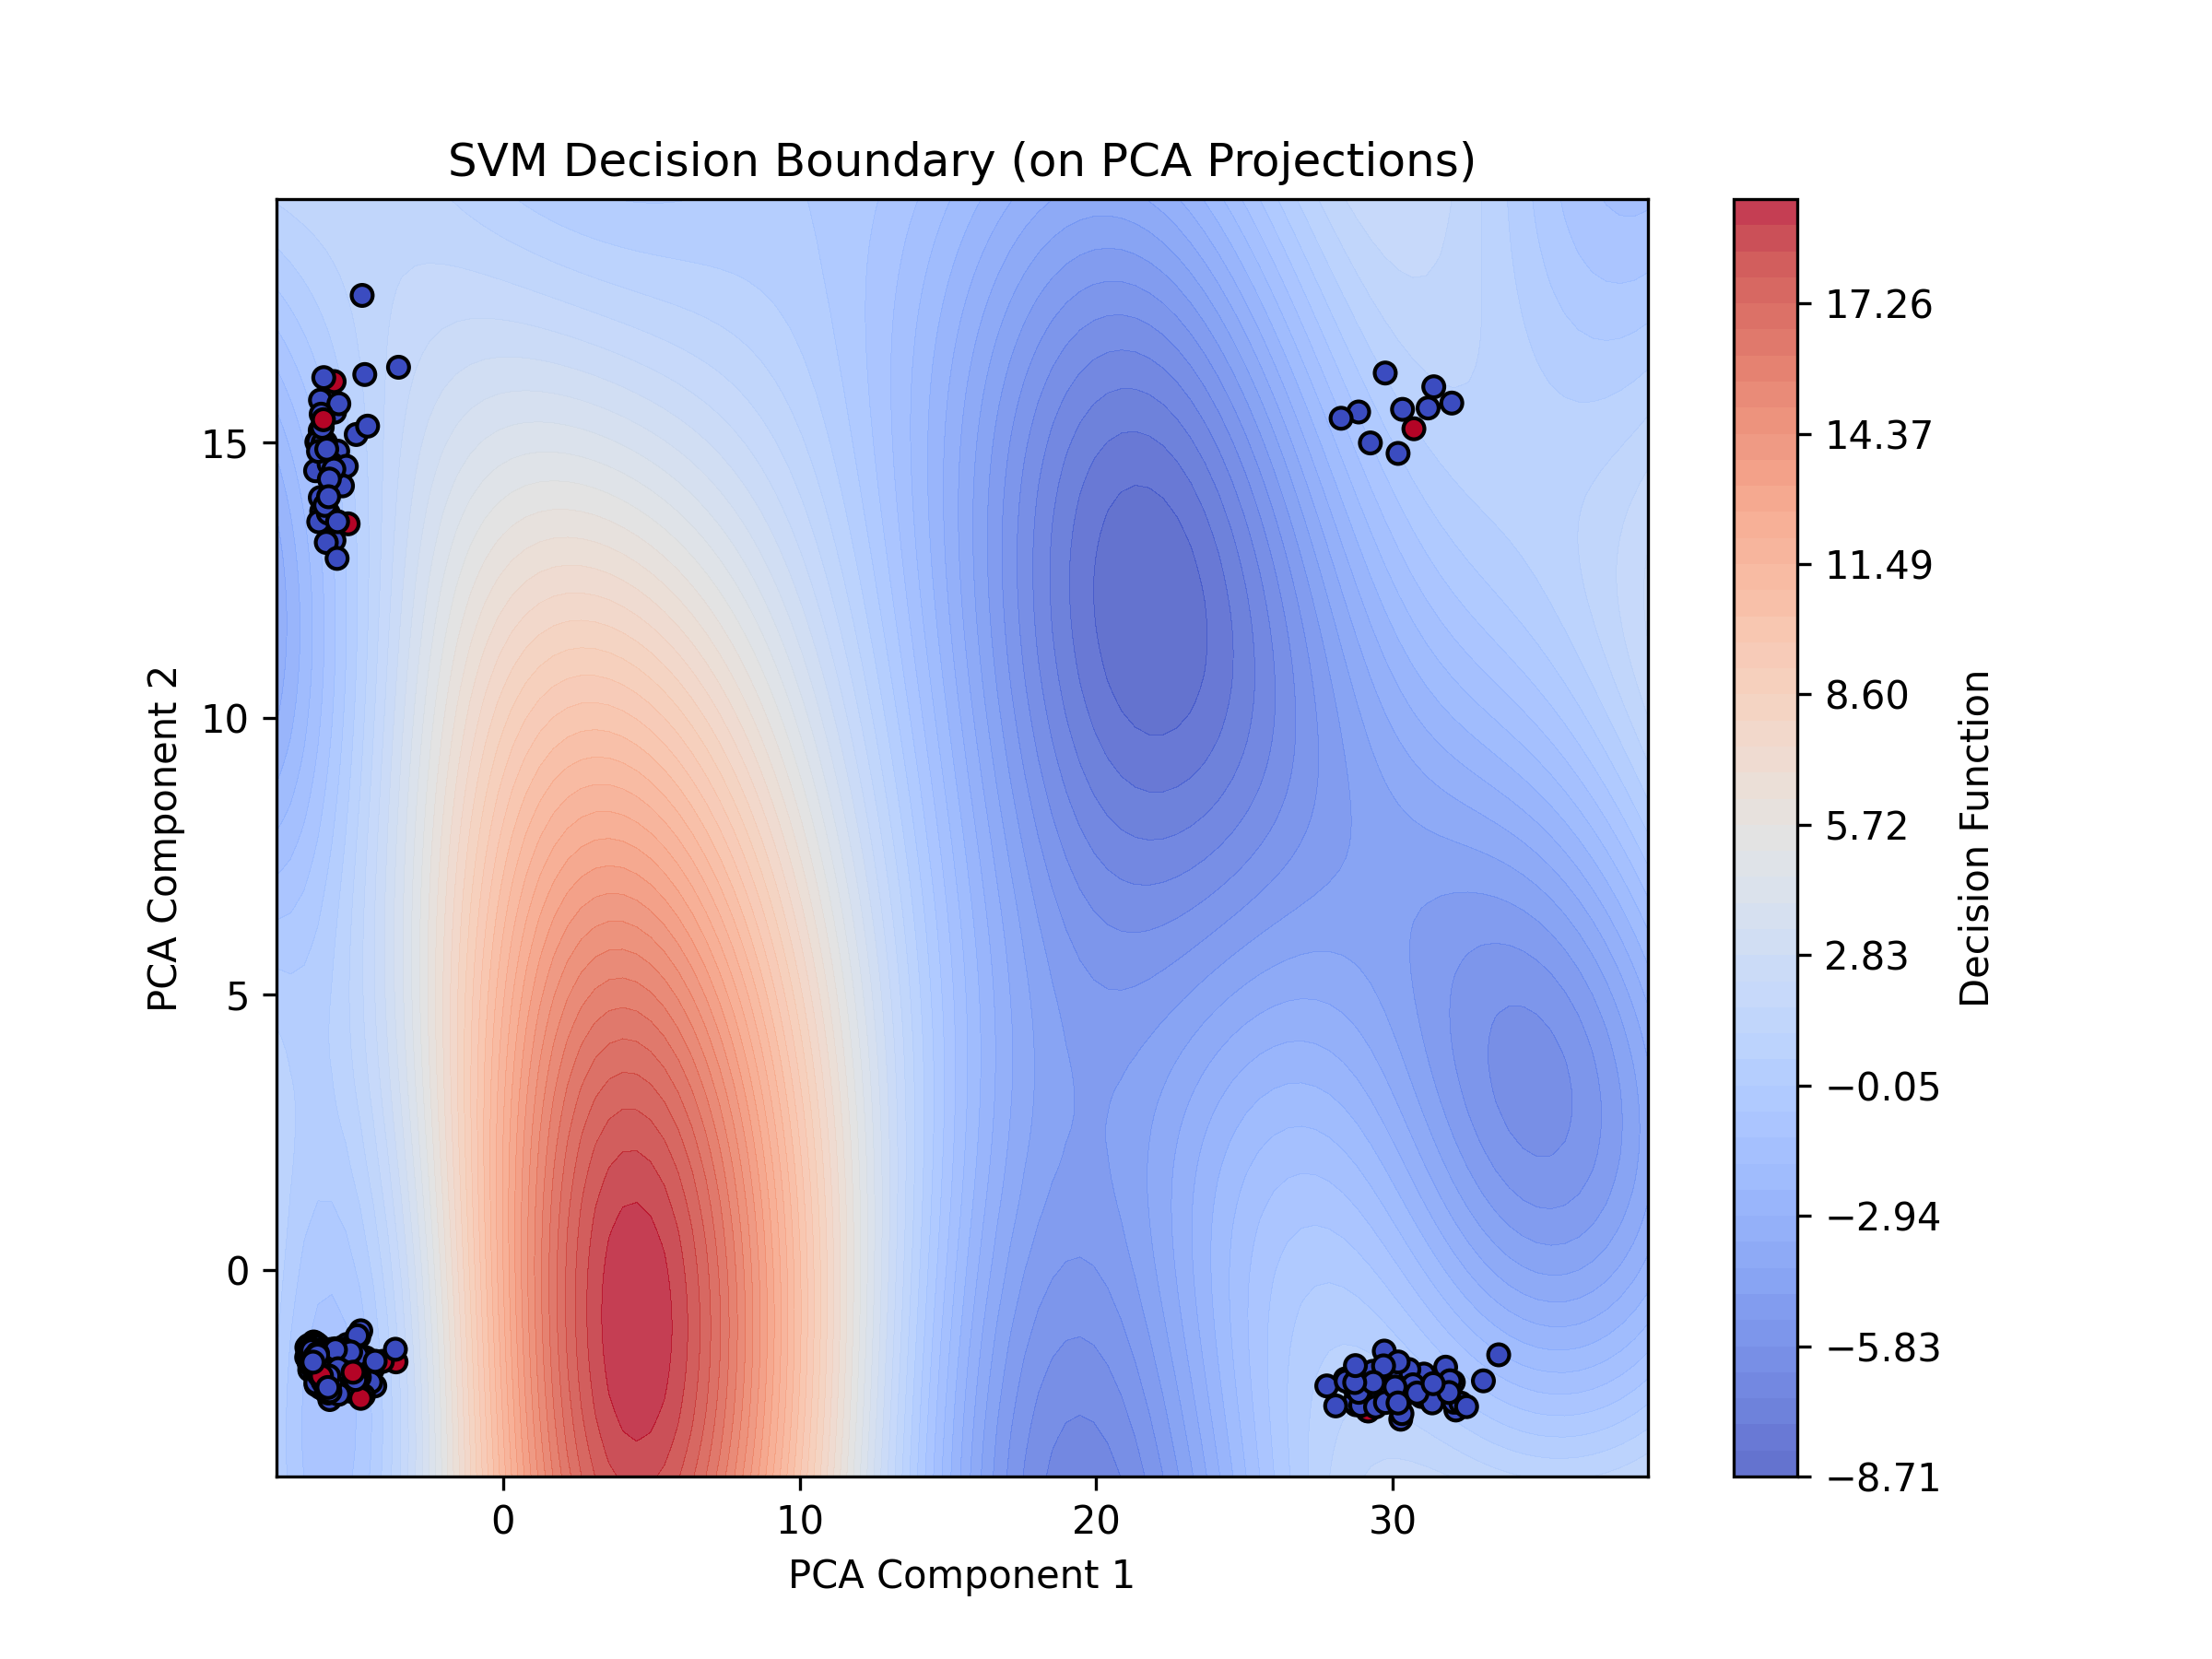
\includegraphics[width=9cm]{plots/svm_decision.png}
\caption{A plot of SVM's decision boundary using PCA projections}%
\label{fig:svm_decision}
\end{figure}


\subsection{Machine Learning Models}
We've tried a handful of different ML models when dealing with the data, including the classic logistic regression, SVM, and PCA/LPCA. Below is a table of the performance of all different models. The training data also uses SMOTE for oversampling to balance the training set. The accuracy, precision, recall and f1-score is measured on a separate test-set after training the model on the training set. All models are tuned to select their best set of hyperparameters using 3 folds cross-validation. Noticably LightGBM model managed to figured out all cases correctly except one in the testing set, which is really impressive.

\begin{table}[H]
\centering
\footnotesize
\begin{tabular}{lllll}
\toprule
\textbf{Model} & \textbf{Accuracy} & \textbf{Precision} & \textbf{Recall} &  \textbf{F1-Score}\\
\midrule
LightGBM & 1.00 & 1.00 & 0.99 & 0.99  \\
Logistic Regression with Regularization & 1.00 & 1.00  & 0.99 & 0.99  \\
Xgboost & 1.00 & 0.99 & 0.98 & 0.97  \\
CatBoost & 0.99 & 0.94  & 0.96 & 0.97  \\
Linear Regression & 0.97 & 0.90  & 0.83 & 0.78  \\
Random Forest & 0.94 & 0.62  & 1.00 & 0.77  \\
\bottomrule
\end{tabular}
\caption{Performance of Different ML Models on the Test Set}%
\end{table}

\begin{figure}[H]
    \centering
    \begin{minipage}{0.32\textwidth}
        \centering
        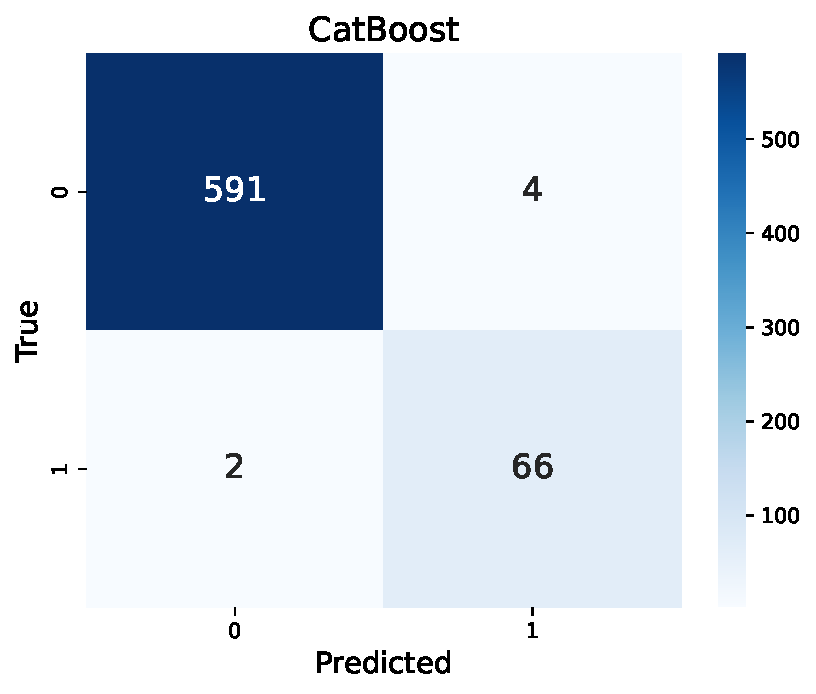
\includegraphics[width=\linewidth]{plots/cb_confusion_matrix.pdf}
        \caption{CatBoost}
        \label{fig:cm-cb}
    \end{minipage}\hfill
    \begin{minipage}{0.32\textwidth}
        \centering
        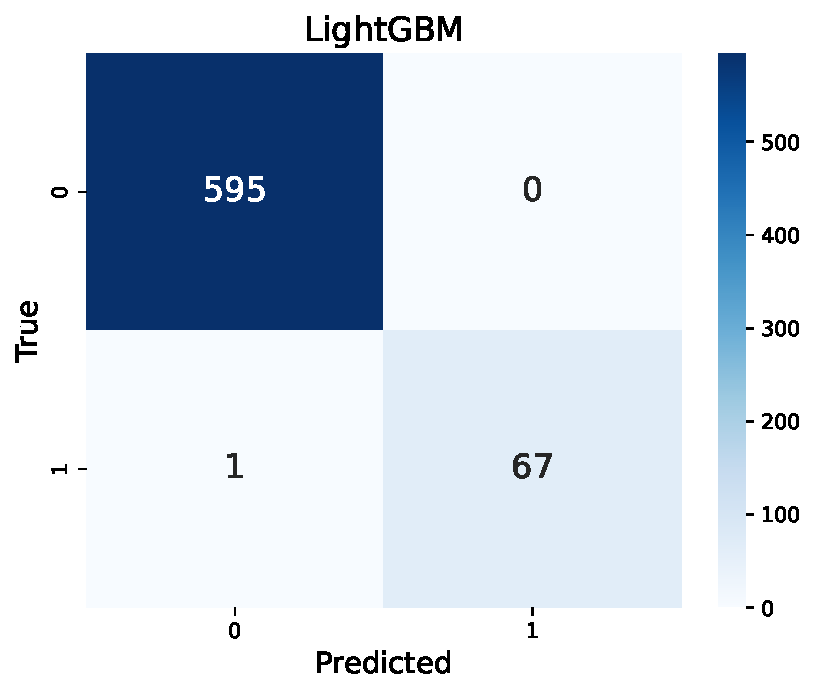
\includegraphics[width=\linewidth]{plots/lgbm_confusion_matrix.pdf}
        \caption{LightGBM}
        \label{fig:cm-lgbm}
    \end{minipage}\hfill
    \begin{minipage}{0.32\textwidth}
        \centering
        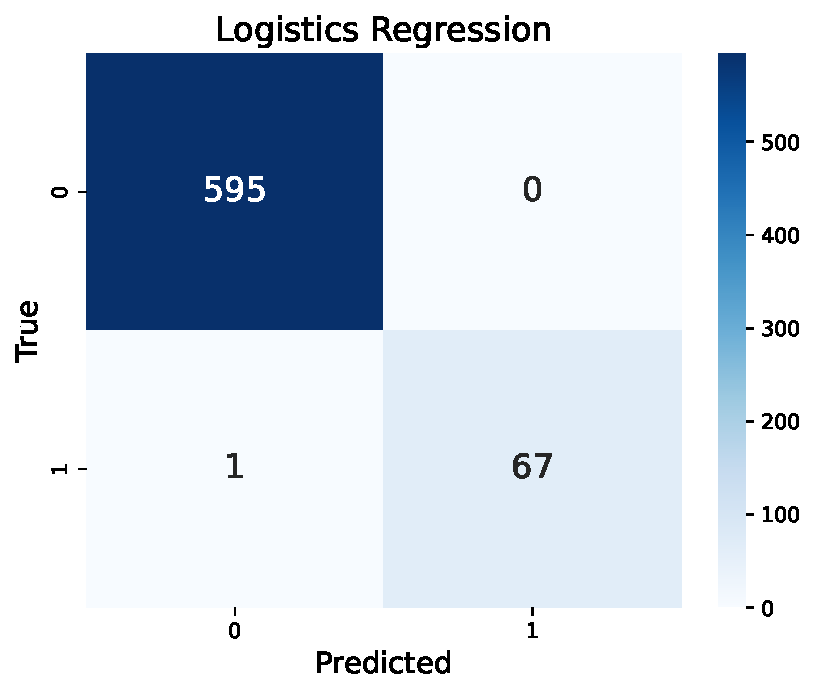
\includegraphics[width=\linewidth]{plots/lgs_reg_confusion_matrix.pdf}
        \caption{Logistic Regression}
        \label{fig:cm-lgs_reg}
    \end{minipage}
    \vspace{1em}
    \begin{minipage}{0.32\textwidth}
        \centering
        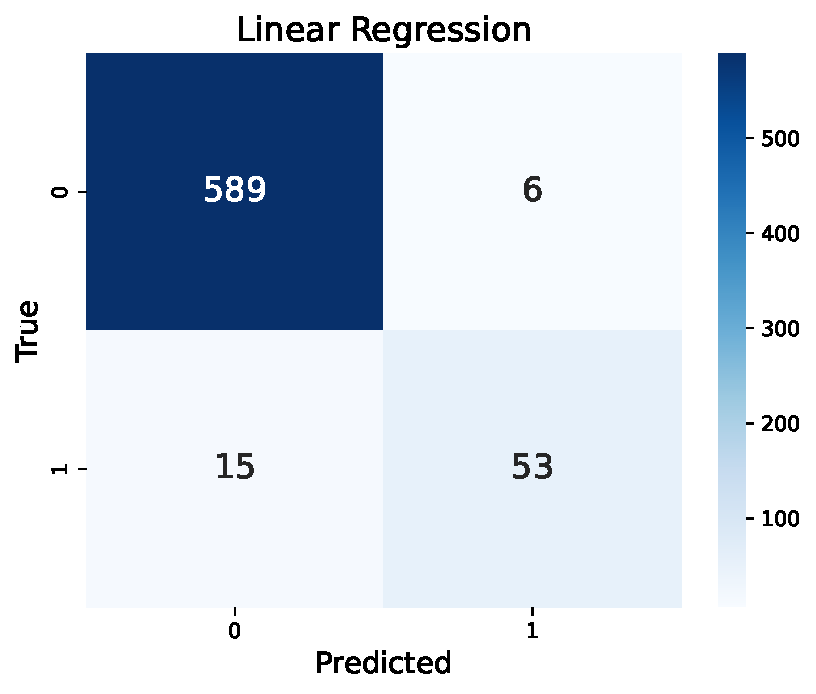
\includegraphics[width=\linewidth]{plots/linear_confusion_matrix.pdf}
        \caption{Linear Regression}
        \label{fig:cm-linear}
    \end{minipage}\hfill
    \begin{minipage}{0.32\textwidth}
        \centering
        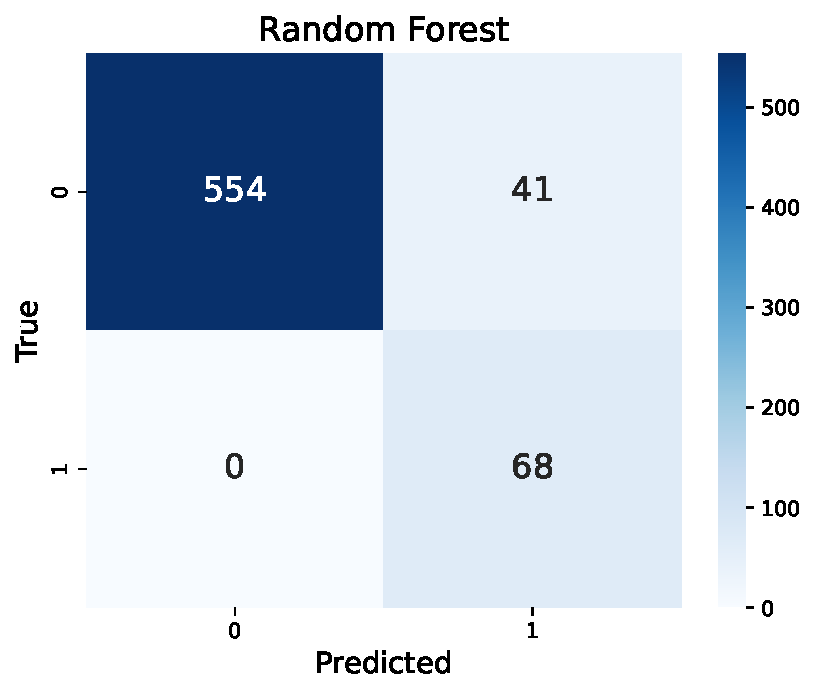
\includegraphics[width=\linewidth]{plots/random_forest_confusion_matrix.pdf}
        \caption{Random Forest}
        \label{fig:cm-random-forest}
    \end{minipage}\hfill
    \begin{minipage}{0.32\textwidth}
        \centering
        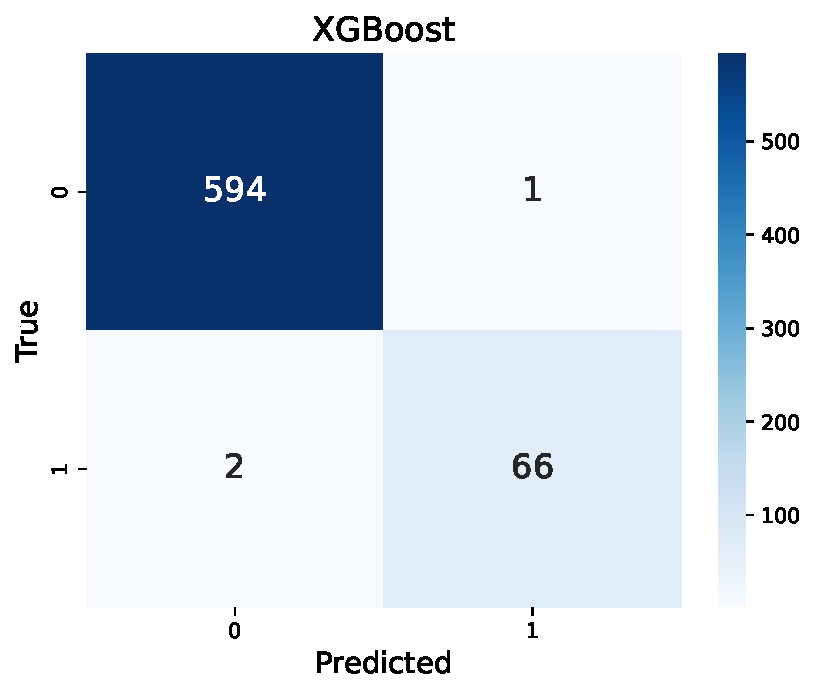
\includegraphics[width=\linewidth]{plots/xgboost_confusion_matrix.pdf}
        \caption{XGBoost}
        \label{fig:cm-xgboost}
    \end{minipage}
    \caption{Confusion Matrices of Different ML Models}
\end{figure}



\subsection{Neural Network models}

For the Neural Network approach, we choose three different approaches: A fully connected multi-layer perceptron (MLP) model, Transformer based TabPFN classification model, and 1D CNN model. 

The MLP implementation consisted on a simple Feed-Forward Neural Network with the following structure:

\begin{table}[H]
\centering
\footnotesize
\begin{tabular}{lllll}
\toprule
\textbf{Layer} & \textbf{Number of nodes} & \textbf{Details} \\
\midrule
Linear & num features * 512 & \\
Dropout &  & 0.2 \\
Linear& 512 * 128 & \\
Dropout & & 0.2 \\
Linear & 128 * 1 & \\
Sigmoid & & \\
\bottomrule
\end{tabular}
\caption{MLP architecture}
\end{table}

The optimizer choice was Adam, based on the versatility and stability on this approach. 
The loss function used is BCEWithLogitsLoss, with the weight of the inverse of frequency of the 
label, to try to balance the data. A learning rate scheduler was implemented to push the model to 
keep learning and find a local minimum. A Early Stopper approach was implemented as well to avoid 
over-fitting if the model is not reducing the loss. In Figure \ref{fig:nn-loss}, the training and
validation loss history is shown. As observed, the total number of epochs was 55, with a patience of 10 epochs.
The model has early stopped the training as the validation loss was not decreasing.

\begin{figure}[H]
    \centering
    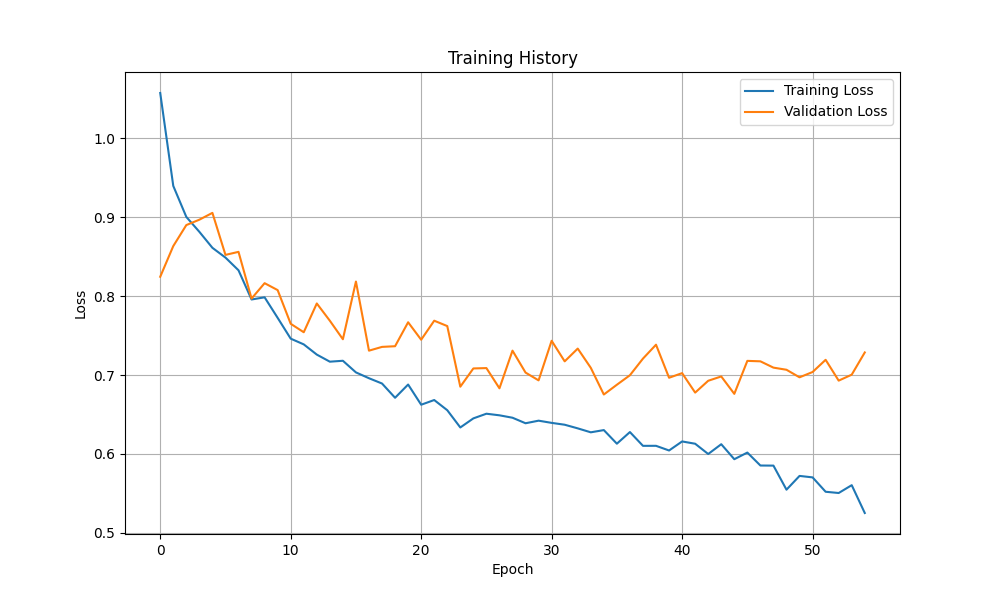
\includegraphics[width=0.5\linewidth]{../plots/NN_loss_graph.png}
    \caption{Training and Validation Loss History}
    \label{fig:nn-loss}
\end{figure}

The confusion matrix obtained by the model is shown below in Figure \ref{fig:cm-nn}. 
We can observe that the model is not able to generalize well, as the number of False Negatives is
higher than the number of True Positives.

\begin{figure}[H]
    \centering
    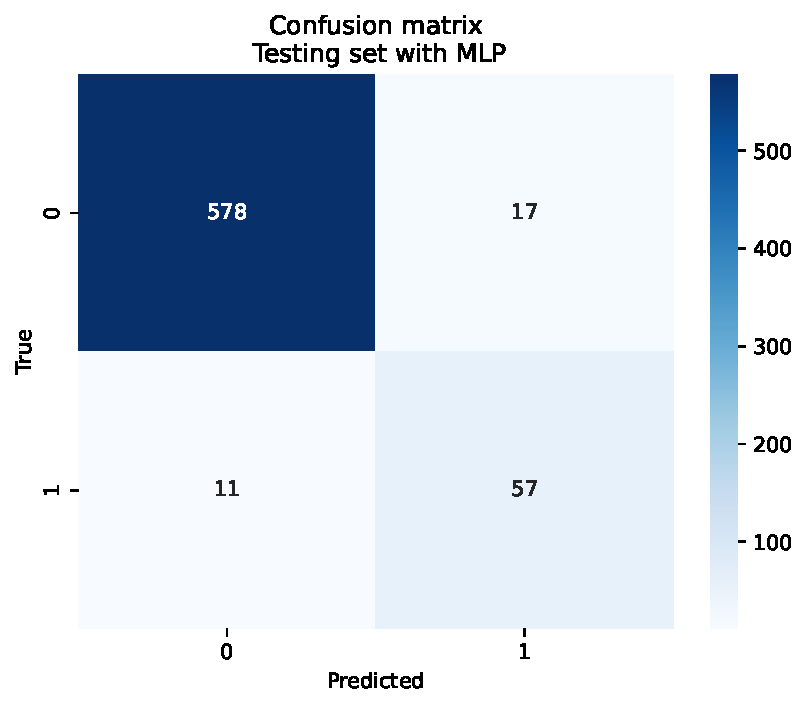
\includegraphics[width=0.5\linewidth]{plots/nn_confusion_matrix.pdf}
    \caption{Confusion Matrix - MLP}
    \label{fig:cm-nn}
\end{figure}

The results of this model, using our choice of metrics, along with the specificity and sensitivity is shown in the table below:

\begin{table}[H]
\centering
\footnotesize
\begin{tabular}{lllll}
\toprule
\textbf{Precision} & \textbf{Recall} & \textbf{Accuracy} &  \textbf{F1-Score}\\
\midrule
0.786 & 0.867 & 0.962 & 0.825  \\
\bottomrule
\end{tabular}
\caption{Performance of MLP on Test Set}%
\end{table}

The transformer implementation is based on Transformer Prediction Framework, referenced in the following paper \cite{hollmann2022tabpfn}. 
The model is based on in-context learning, where the tabular data is inferred by pretrained transformer, 
and then uses Bayessian updates to infer the posterior distribution of the prediction and parameters based on the 
new information. The model is trained on the same data as the Vanilla Neural Network, with the same data splitting and resampling.

The proposed approach is significantly better than the Vainilla approach, as it can reduce both 
the specifiticity and sensitivity, as shown in the confusion matrix below.

\begin{figure}[H]
    \centering
    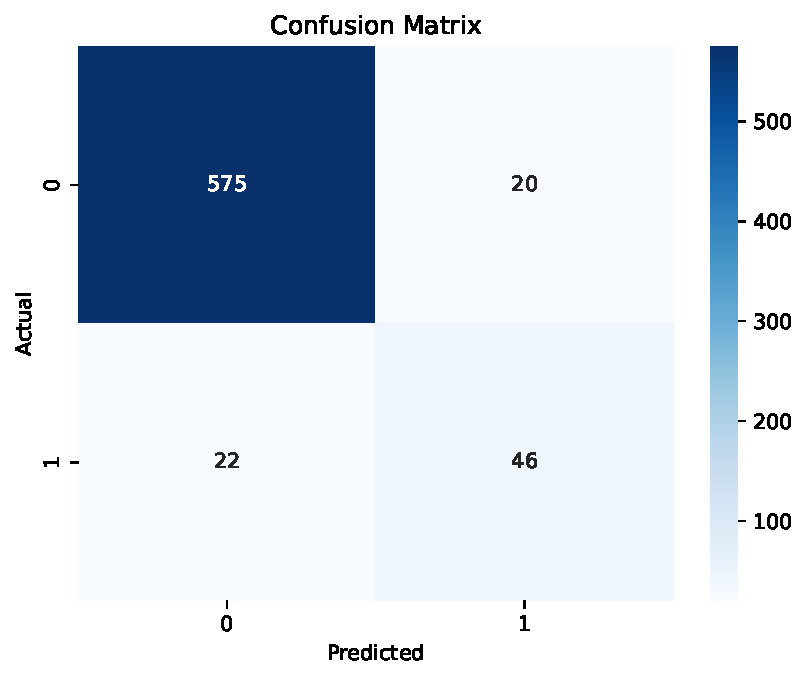
\includegraphics[width=0.5\linewidth]{plots/tabpfn_confusion_matrix.pdf}
    \caption{Confusion Matrix of TabPFN on Testing data}
    \label{fig:confusion-matrix-transformer}
\end{figure}

The results and the metrics of this model is shown below:

\begin{table}[H]
\centering
\footnotesize
\begin{tabular}{lllll}
\toprule
\textbf{Sensitivity} & \textbf{Specificity} & \textbf{Accuracy} &  \textbf{F1-Score}\\
\midrule
0.6760 & 0.966 & 0.9325 & 0.6865  \\
\bottomrule
\end{tabular}
\caption{Performance of Transformer Implementation}%
\end{table}

As observed, the Transformer model is significantly better than the Vanilla Neural Network, or any Machine Learning model.
The Transformer model not only outperforms the other models in terms of F1-Score, but also maintains a high specificity and sensitivity.
Additionally, the False Negative Rate (FNR) is significantly lower than the other models. 

We have also tried using a 1D CNN model to do data classification. Leveraging the translational equivariance property of CNNs, the model can capture locational features between neighboring columns inside the dataset. Since a lot of our data has very high correleation to its neighboring column, the model can utilize this information and do classifications based on that.

There's a good amount of stuff still open to further dicussion and testing, including the use of MaxPooling to do dimension reduction, number of channels for the convolution layers and the kernal size. So far we've selected the parameters based on performance of f1-score on the validation set.

\begin{table}[H]
\centering
\footnotesize
\begin{tabular}{lllll}
\toprule
\textbf{Layer} & \textbf{Number of nodes} & \textbf{Details} \\
\midrule
Linear & num features * 1024 & \\
Dropout & & 0.2 \\
Conv1D & in channel = 16, out channel = 16 & kernal size=5\\
MaxPool1D &  & kernal size=2\\
Conv1D & in channel = 16, out channel = 16 & kernal size=5\\
MaxPool1D & & kernal size=2\\
Conv1D & in channel = 16, out channel = 16 & kernal size=5\\
MaxPool1D & & kernal size=2\\
Linear & 64 * 16 & \\
Linear & 16 * 1 & \\
Sigmoid & & \\
\bottomrule
\end{tabular}
\caption{1D CNN model architecture}
\end{table}
It turns out to be that 1D-CNN models has so far the best result for neural network approach for doing the binary classification. The results and metrics is shown below:

\begin{table}[H]
\centering
\footnotesize
\begin{tabular}{lllll}
\toprule
\textbf{Precision} & \textbf{Recall} & \textbf{Accuracy} &  \textbf{F1-Score}\\
\midrule
0.780 & 0.882 & 0.962 & 0.827  \\
\bottomrule
\end{tabular}
\caption{Performance of 1D CNN on Test Set}%
\end{table}

\begin{figure}[H]
    \centering
    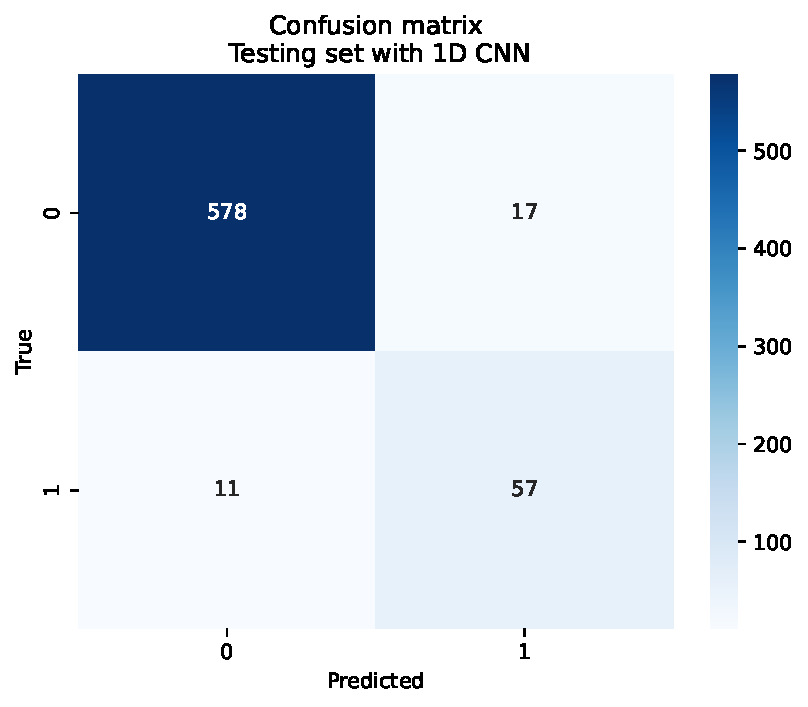
\includegraphics[width=0.5\linewidth]{plots/1dcnn_confusion_matrix.pdf}
    \caption{Confusion Matrix of 1D CNN on Testing data}
    \label{fig:confusion-matrix-1dcnn}
\end{figure}

\subsection{Final Selection of Model}
We've finally selected the LightGBM model, as it demonstrated exceptional result in doing the actual classification. Due to it's built upon decision trees as the base learner, it's easier for us to interpret the model and understand the decision making process. The model is also very fast to train and can be easily implemented in a production environment. Below is the decision process of the model:

\begin{figure}[H]
    \centering
    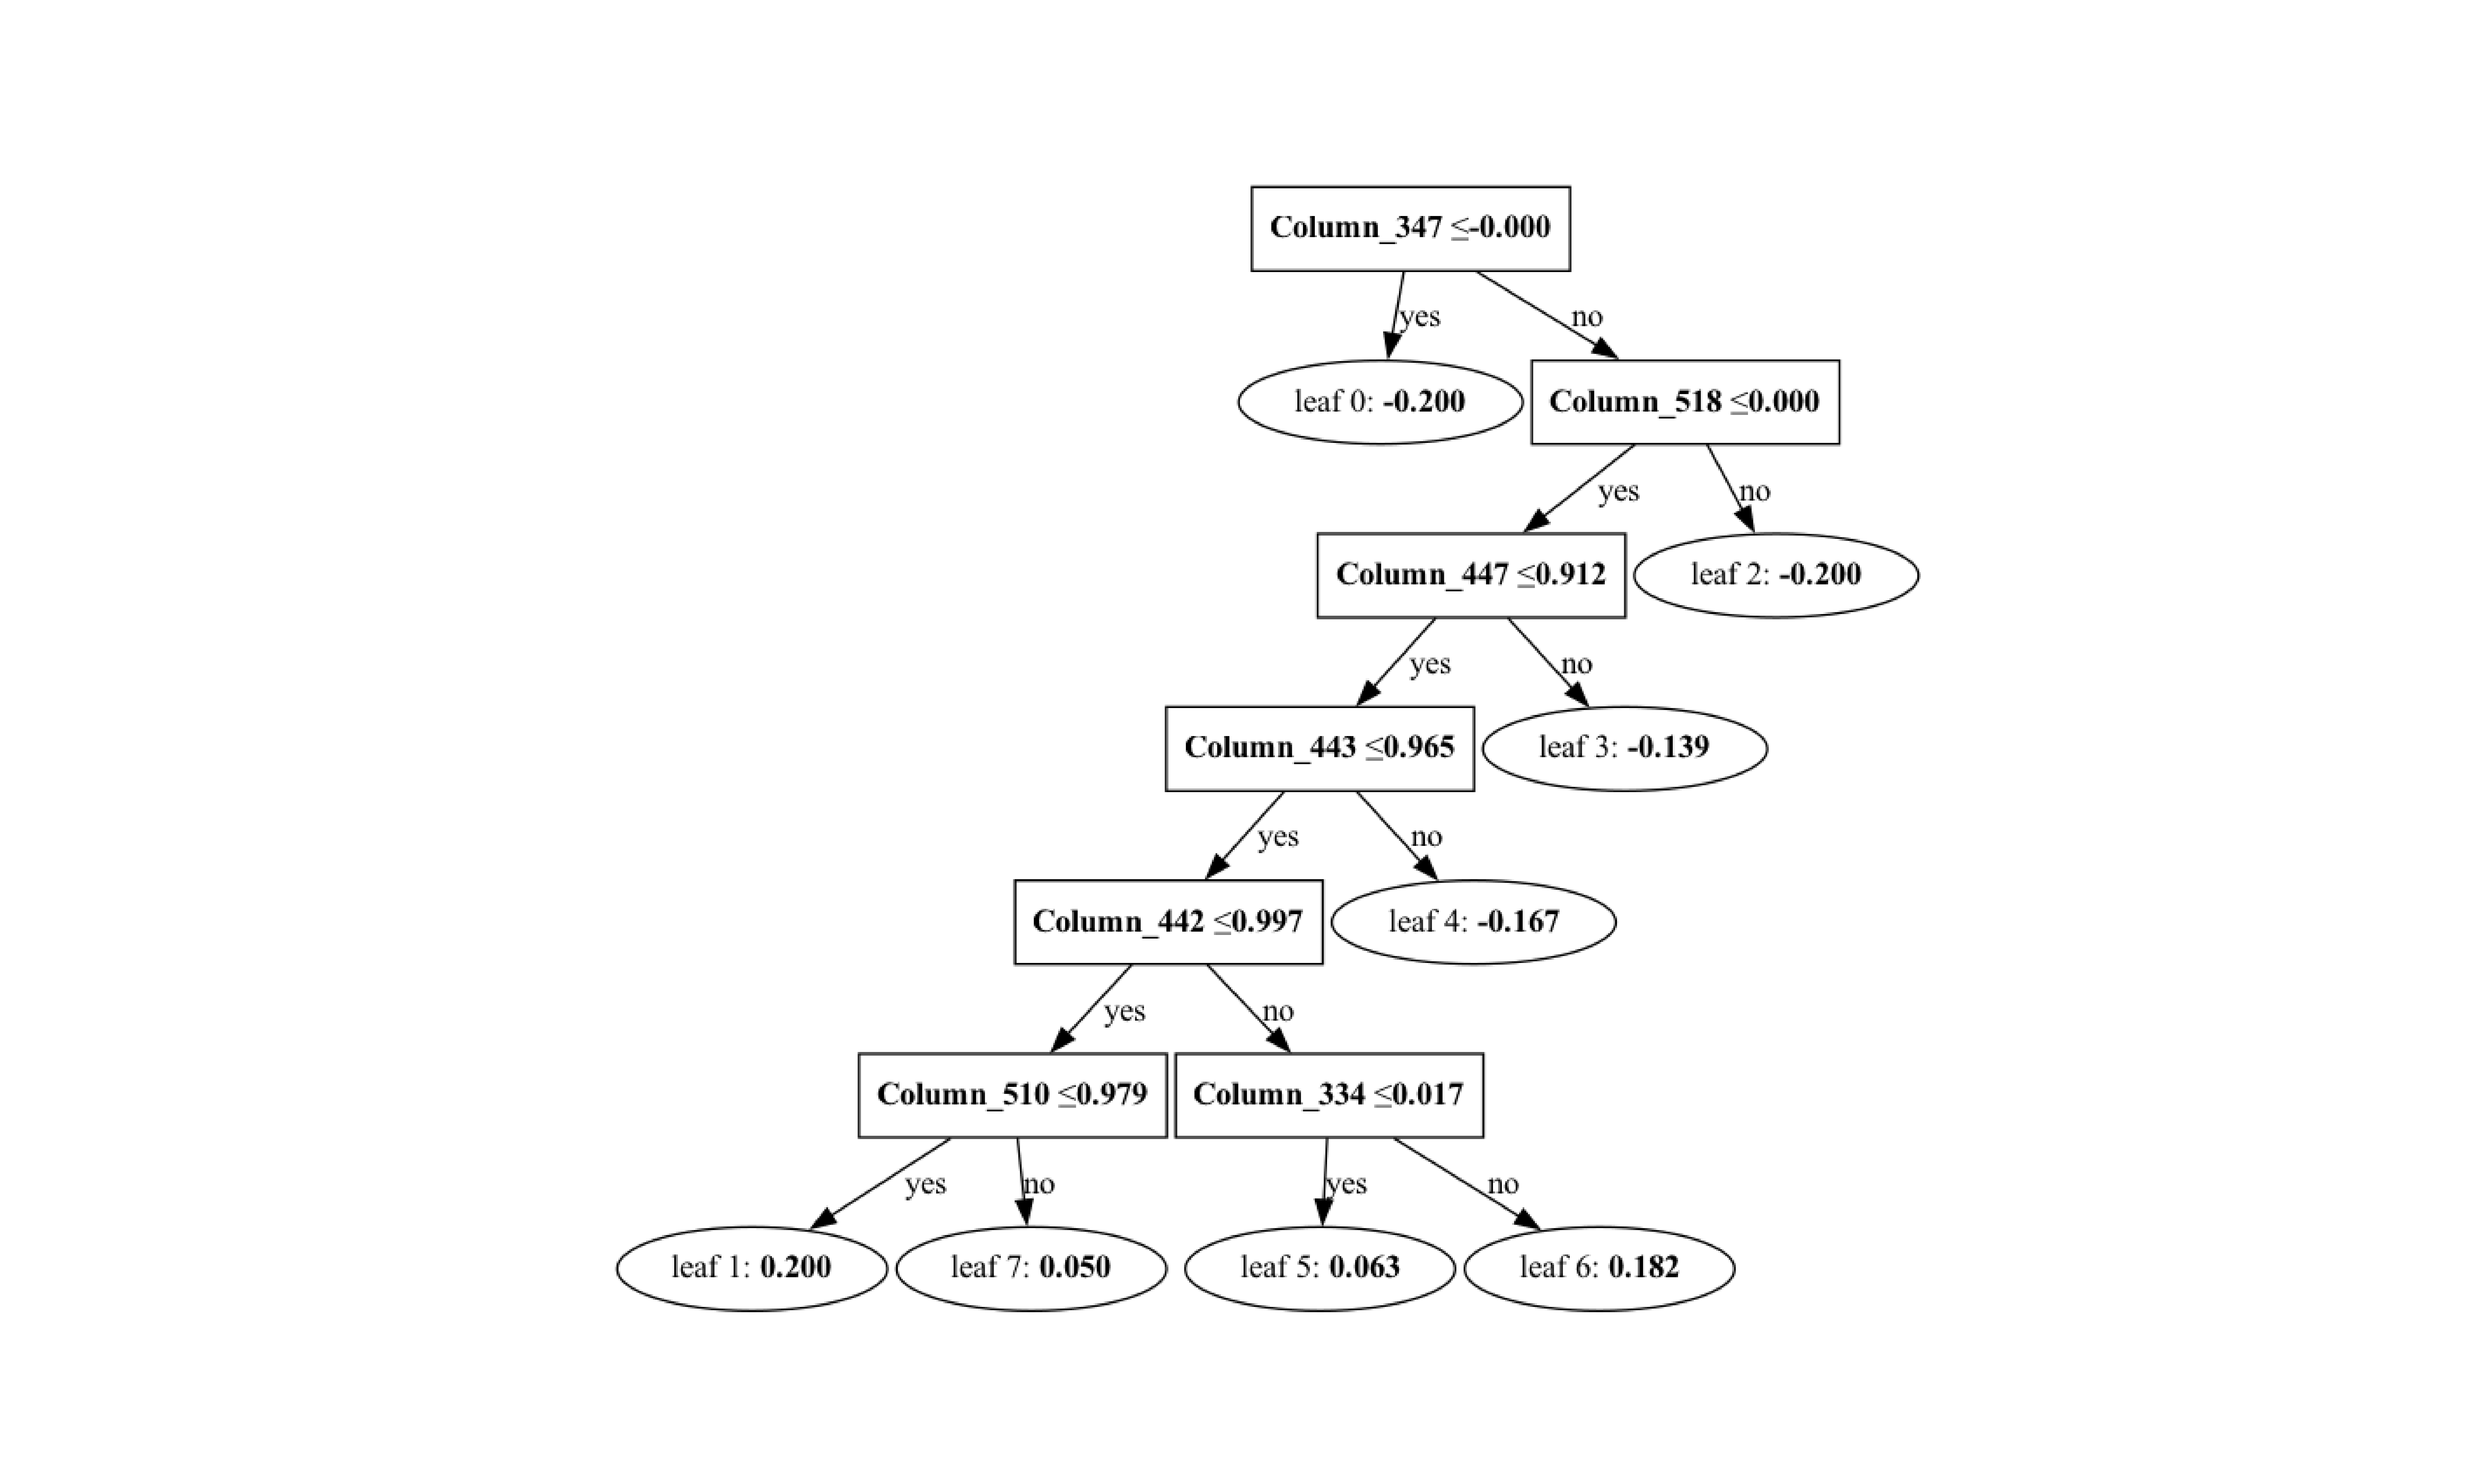
\includegraphics[width=\linewidth]{plots/lgbm_tree_vert.pdf}
    \caption{The decision making process of LightGBM model}
    \label{fig:confusion-matrix-transformer}
\end{figure}

Here's a table of columns referring to the decision making process of the model:

\begin{table}[H]
    \centering
    \footnotesize
    \begin{tabular}{lll}
    \toprule
    \textbf{Column Name} & \textbf{Label} & \textbf{Description} \\
    \midrule
    347 & CFracturesOC & Occipital condyle fracture \\
    518 & CordInjuryNoRadiographic & Does the patient have a spinal cord injury without radiographic association?\\
    447 & C1\_2SbLigSLARS & C1-2 atlantoaxial rotary subluxation\\
    443 & LigamentousInjuryOAD & Cccipital-atlantal dislocation \\
    442 & Ligamentoptions & Were there ligamentous injuries to the cervical spinal column? \\ 
    510 & OperativeReport & Was a spine surgery operative report available? \\ 
    \bottomrule
    \end{tabular}
    \caption{Columns used in the decision making process of LightGBM model}%
\end{table}

LightGBM does not assume the closer a node is to the root, the more important it is. It's generally selecting the most important features to split on, and the feature importance is calculated based on the number of times a feature is used to split the data. Clearly that the selected columns play a crucial role in dividing up all different forms of data, and most of them are from the Injury classification document. 

\section{Interpretability}

Additinally, we have observed the use of the Transformer as a feasible model for the decision rule. This section will address if our model is interpretable to provide
trust and confidence to the medical practitioners. The model is based on the Tabular Prediction Framework (TabPfn) \cite{hollmann2022tabpfn}, 
which relies on the prior training on sequential data. However, as any Deep Learning model, the model is a black box,
and it is hard to interpret the features and its importance. 

However, according to Rundel et al. \cite{rundel2024interpretable}, they proposed a set tools to interpret the results of the model.
In this case, we will implement a Decision Curve Analysis (DCA) to understand the model's decision making process.

\begin{figure}[H]
    \centering
    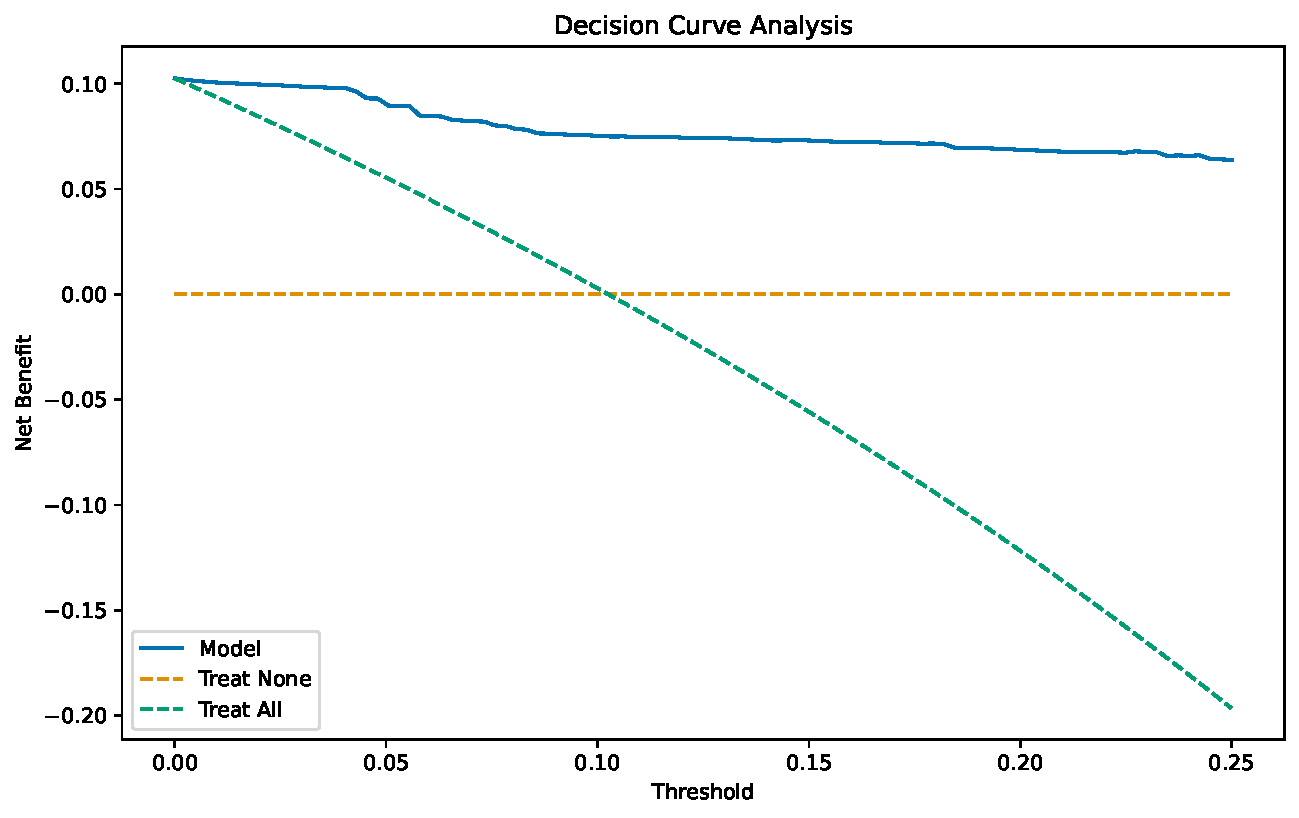
\includegraphics[width=0.5\linewidth]{../plots/tabpfn_decision_curve.pdf}
    \caption{Decision Curve Analysis}
    \label{fig:dca}
\end{figure}

This plot helps use realize how the model improves for intervention all the time, where the model inferes that even if the threshold is high, it is smart to not 
always decide to immobilize the patient \cite{vickers2019simple}. In this case, the threshold 
represents the amount of worry the model has to have to decide to immobilize the patient. Therefore, this graph 
can help the medical practitioners to understand the model's decision making process.

However, this implementation does not uncover the overall importance of the features, just how the model is making the decision.
This is a main drawback for the model, as the medical practitioners might not trust the model if they do not understand how the model is making the decision.
Hopefully, in a real world application, using expert notions and domain knowledge, the input feature space of the model can 
be reduced to a more interpretable space, and the model can be used as a decision rule.

\section{Stability}
\subsection{Model Perturbation}
The model perturbation ablation setup starts from the parameter tuning stage, which when we were doing hyperparameter tuning, we used 3 fold cross-validation to select the best set of hyperparameters. The model might have some structural difference since the number of depth is changing, the overall performance is not changing significantly (as of overfitting super bad or underfitting). The model itself is still capable of generalizing, though the performance might be slightly different but not affecting that much.

An example for this would be if we use depth of 2 instead of 6 for the LightGBM model, the f1 score drops to 0.93 from 0.99. However, the model is still capable of generalizing and predicting the correct value.

For the model perturbation in the Transformer, we tried the following:
\begin{itemize}
    \item Train the model with a different loss function, e.g. Categorical Cross-Entropy, to see if the model can generalize well.
    \item Train the model with different set of hyperparameters, by using a different set of learning rate, batch size, and number of epochs.
\end{itemize}

The results of the model perturbation is shown below:

\begin{table}[H]
\centering
\footnotesize
\begin{tabular}{lllll}
\toprule
\textbf{Model} & \textbf{Accuracy} & \textbf{Precision} & \textbf{Recall} &  \textbf{F1-Score}\\
\midrule
Model & 0.50 & 0.81  & 0.90 & 0.85  \\
Model (Different Loss) & 0.489 & 0.745  & 0.89 & 0.745  \\
Model (Different Hyperparameters) & 0.475 & 0.704  & 0.875 & 0.812  \\
Model (Different number of PCA components) & 0.415 & 0.652 & 0.90 & 0.65  \\
\bottomrule
\end{tabular}
\caption{Performance of Different Perturbations}%
\end{table}

As shown, the model seems to be stable under model choices. However, we might not be entirely sure if the model is stable under different
data perturbations. Therefore, we will proceed to the next section to analyze the data perturbation.

\subsection{Data Perturbation}
Note: We've tried doing data perturbation using LightGBM, but the results are not really interesting enough 
(the f1-score and accuracy are not dropping drastically). From here we went with TabPFN method 
(we also just want to use something different as well to see how it performs), which shows something 
more interesting in terms of the performance. \\

The setup of data perturbation is mainly comparing the inline distribution disparity between different sites. 
However, this implies that the sites are independent and relies on the same proportion of prevalence (or imbalance), 
which might not be true in real world. Therefore, we implemented a stability check with the training on high prevalence 
proportion and test on the sites with least cases, to see if we can get the same behavior. We retrained our model and test 
it on the least 5 sites on the data. The number of 5 sites for testing is a \textbf{judgment call}, as the number can 
fluctuate as the data availability becomes scarce or not.  

The confusion matrix is shown below:

\begin{figure}[H]
    \centering
    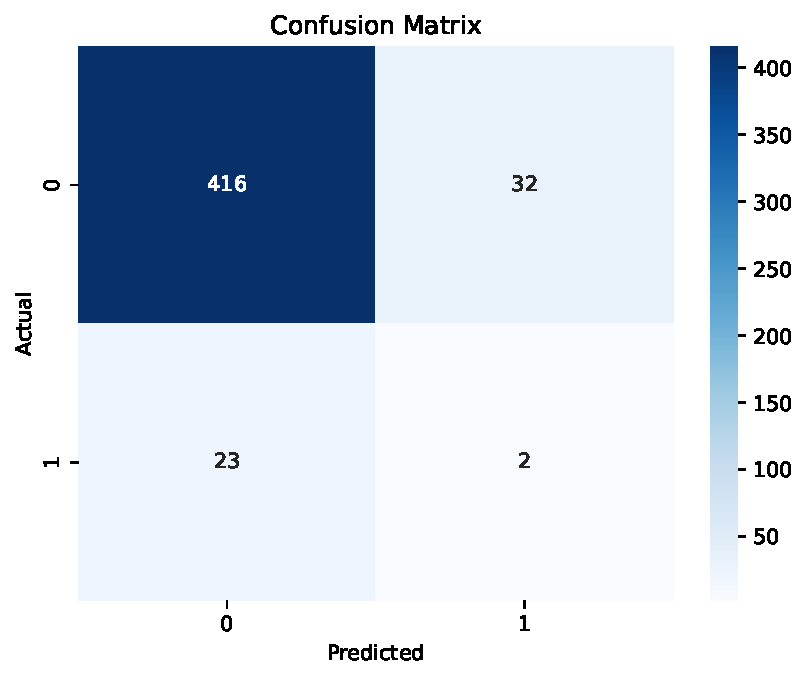
\includegraphics[width=0.5\linewidth]{../plots/tabpfn_confusion_matrix_stab1.pdf}
    \caption{Stability on prevalence}
    \label{fig:stability1}
\end{figure}

As observed, the confusion matrix greatly decrease the number on prediction, as our class weights 
used before does not correspond to the reality of the testing sites. This initial verification can help us 
observe the importance of our assumptions. Therefore, we implemented more investigation by increasing
the number of sites with least proportion out of our training set. The results are shown below:

\begin{figure}[H]
    \centering
    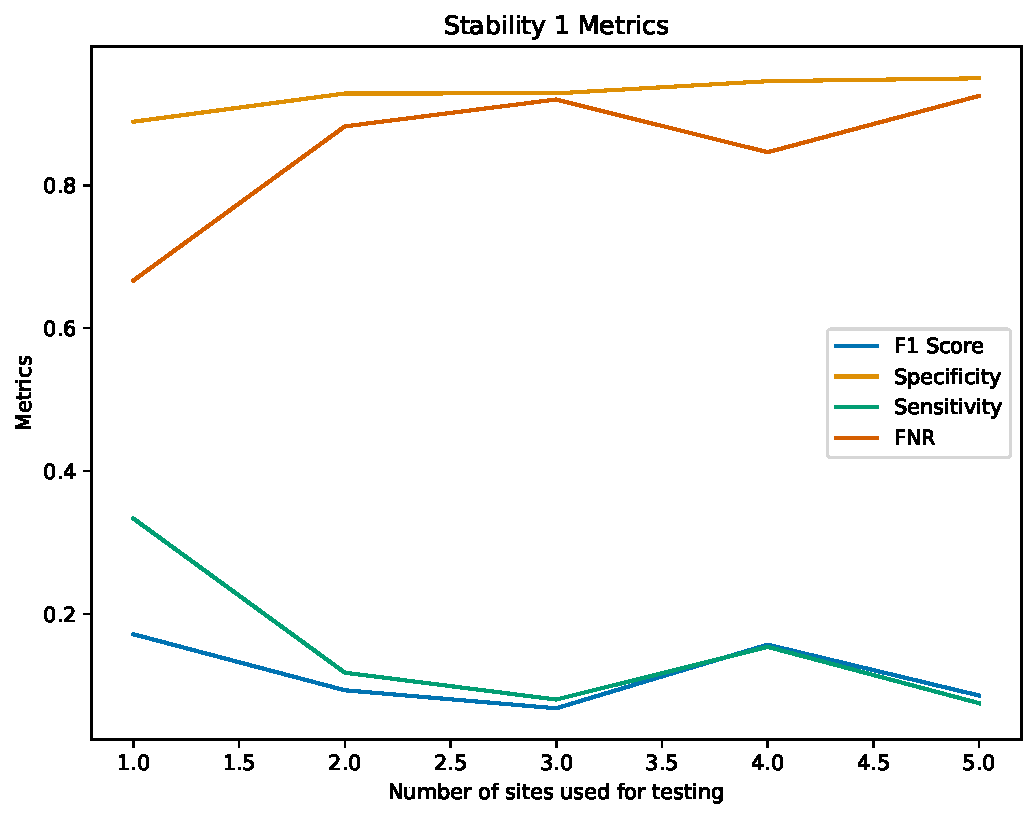
\includegraphics[width=0.5\linewidth]{../plots/tabpfn_stability1_metrics.pdf}
    \caption{Stability on prevalence: Metrics changing}
    \label{fig:stab-1}
\end{figure}

As shown in Figure \ref{fig:stab-1}, the metrics certainly decreases as the prevalence is taking into consideration. However, still our model predicts fairly good estimations of the predicted value, maintaining the specificity and FNR.

Our next data perturbation considers the sub sampling problem of the data. The reality explanation would reference to a medical site where the information is still ongoing, as the number of patients are increasing, and we might not be able to train our model with the full dataset on a given year. 
Therefore, it is important to observe if the model is stable enough to still reproduce good results even at this criteria. 

\begin{figure}[H]
    \centering
    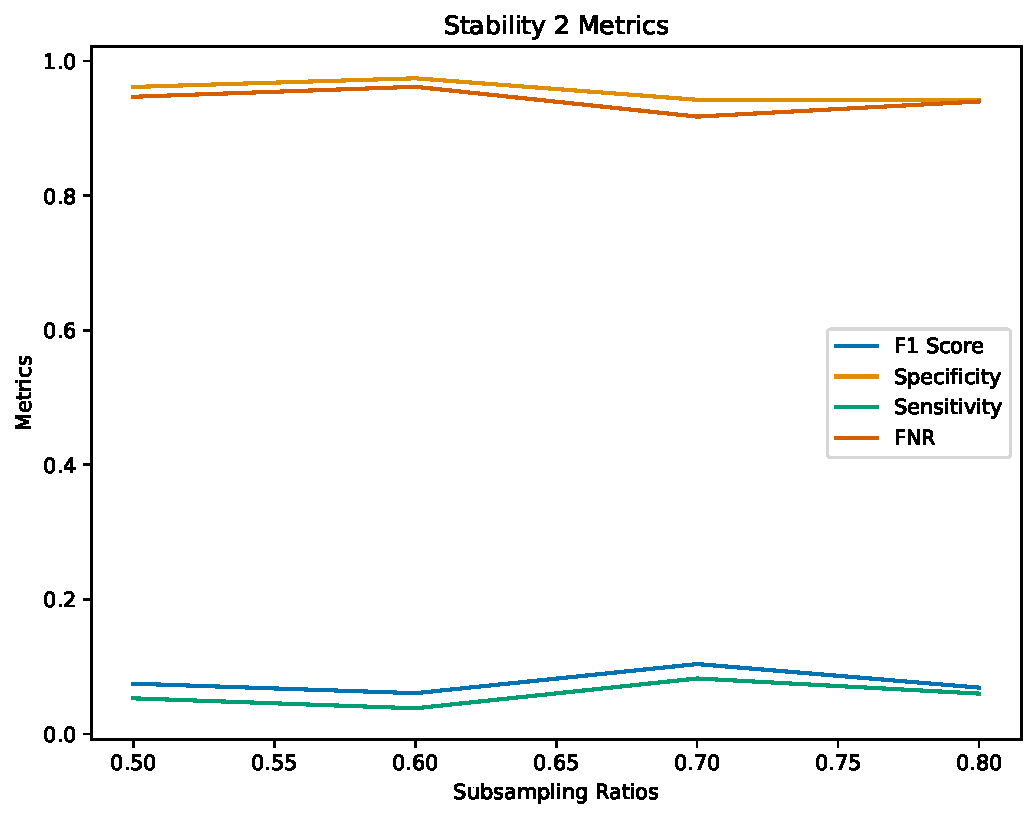
\includegraphics[width=0.5\linewidth]{../plots/tabpfn_stability2_metrics.pdf}
    \caption{Stability on sub sampling: Metrics changing}
    \label{fig:enter-label}
\end{figure}

Additionally, an additional stability analysis have been made, by changing the sampling of the data based on SMOOTE, to see if the model is 
still able to generalize well. The results are shown below:

\begin{figure}[H]
    \centering
    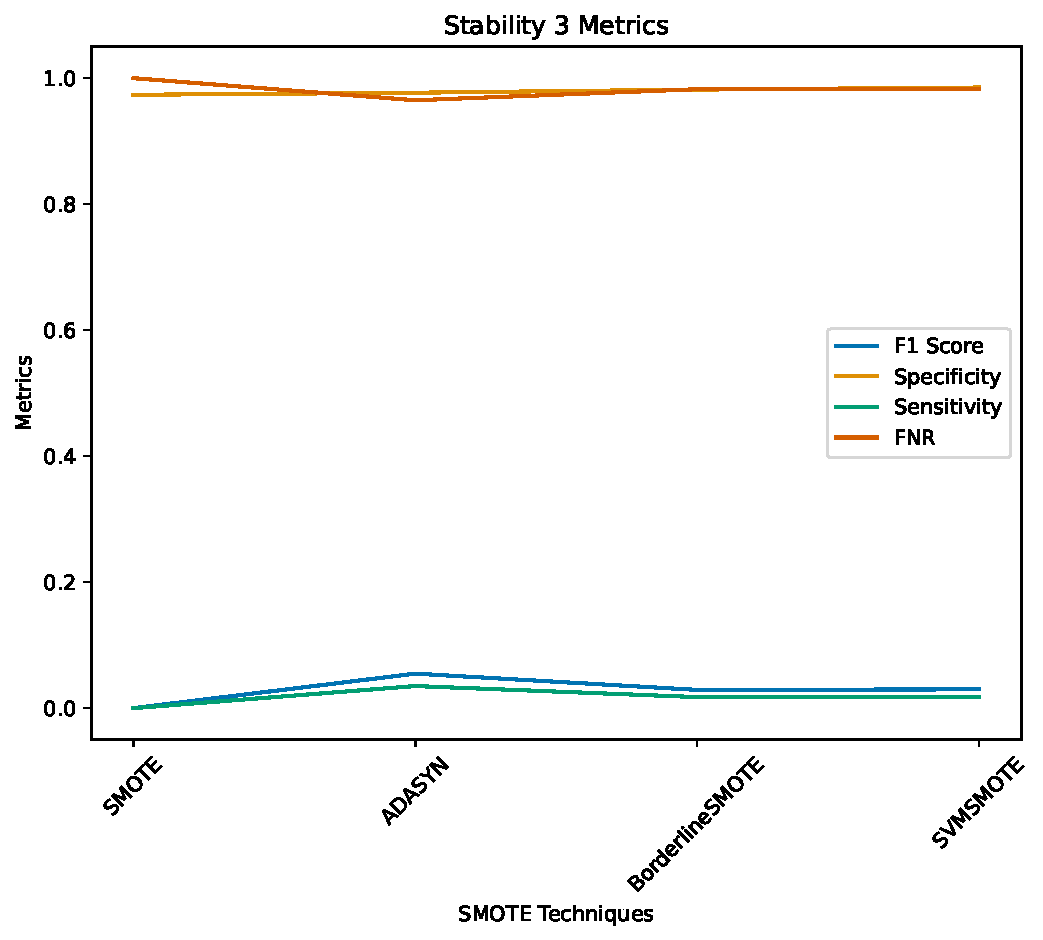
\includegraphics[width=0.5\linewidth]{../plots/tabpfn_stability3_metrics.pdf}
    \caption{Stability on SMOTE: Metrics changing}
    \label{fig:enter-label}
\end{figure}

As shown, the proportion of the data does not affect the model's performance, as the model is still able to generalize well. Although,
an initial drop of the performance is observed. 

\section{Reality Check}

We have developed and evaluated several predictive models aimed at identifying the most effective approach for medical decision-making regarding patient immobilization. Our methodology involved exploring various feature reduction techniques to distill complex data into actionable insights, thereby facilitating informed decisions by medical practitioners. By focusing on the most relevant features, our models provide a concise and accurate assessment of whether immobilization is necessary.

Notably, real-world hospital data often exhibits considerable diversity, which may not be fully captured by 
existing frameworks such as PECARN. Our model addresses this limitation by providing a data-driven summarization
 of key features, enabling hospitals to make more informed decisions. Furthermore, integrating our model with digital
  medical histories and emergency department (ED) signals has the potential to enhance adoption and improve patient outcomes.

Our model demonstrates improved sensitivity and specificity for false negatives (FN) compared to baseline models. 
However, it is essential to acknowledge that our approach relies on the assumption of low prevalence rates, 
which may not hold true in all clinical settings. To address this limitation, we conducted stability analyses, 
highlighting the need for feedback mechanisms to refine our model for extraordinary case scenarios. Ongoing 
collaboration and testing will be crucial in refining our model's performance and generalization.

To answer how our model would be use in a real wolrd scenario, we need to understand that the model have been 
trained by a complete-knowledge dataset, implying we have all the information already at hand. Therefore, 
our clinical decision rule model would be best suited when the patient is already in the hospital, or ED.
The model would be very challenging to explain to a patient, since the model suffers from sufficient 
explanability. However, we believe that the predicted output would be sufficient to reduce the time of the 
patient on the hospital, which can be seen as a good outcome for them.

Following the same line of thought, we believe that the best scenario for our model is a combined approach, 
where the model informs the medical practitioner, and the medical practitioner makes the final decision. 
We do not believe our model can replace the medical practitioner, as the model is not perfect, and the variables
used are not always present in the patient's case.


\newpage
\section{Bibliography}
\bibliographystyle{unsrt}
\bibliography{references} 

\appendix
\section{Academic honesty}
We, the authors, hereby declare that this work presents our original research and results, conducted and interpreted in good faith, following the project instructions. All reviews, results, and figures were independently developed and understood by us. We acknowledge the resources and previous works that informed our research, citing them accordingly. We affirm that the information used is authentic and accurately represented to the best of our knowledge and understanding.

\subsection{Statement}

\subsection{Collaborators}
Anthony Ozerov for helping us settle the correct implementation of the decision rule.

\subsection{LLM Usage}

\subsubsection*{Coding}
Portions of this code were reviewed and suggested by GitHub Copilot LLM, and Anthropic Claude 3.5 Sonnet. However, the original code structure and implementation were created by us. Where applicable, references are provided to maintain the original authorship of any reused or adapted code, ensuring transparency and proper attribution.

\subsubsection*{Writing}
No use of LLM had been used for the elaboration of the text. Some queries were used to understand some topics, but not to write any text.

\section{Training Minutes}
\subsection{LightGBM Decision making process}
The best set of parameters for LightGBM so far is:
\begin{table}[H]
    \centering
    \begin{tabular}{ll}
    \textbf{Parameter} & \textbf{Value} \\
    \hline
    max-depth & 6 \\
    n-estimator & 100 \\
    Learning Rate & 0.1 \\
    \end{tabular}
    \end{table}
The training process is very fast due to parallelism implementation of LightGBM training loop. The decision making process is shown in the figure below:

\newpage
\begin{figure}[H]
    \centering
    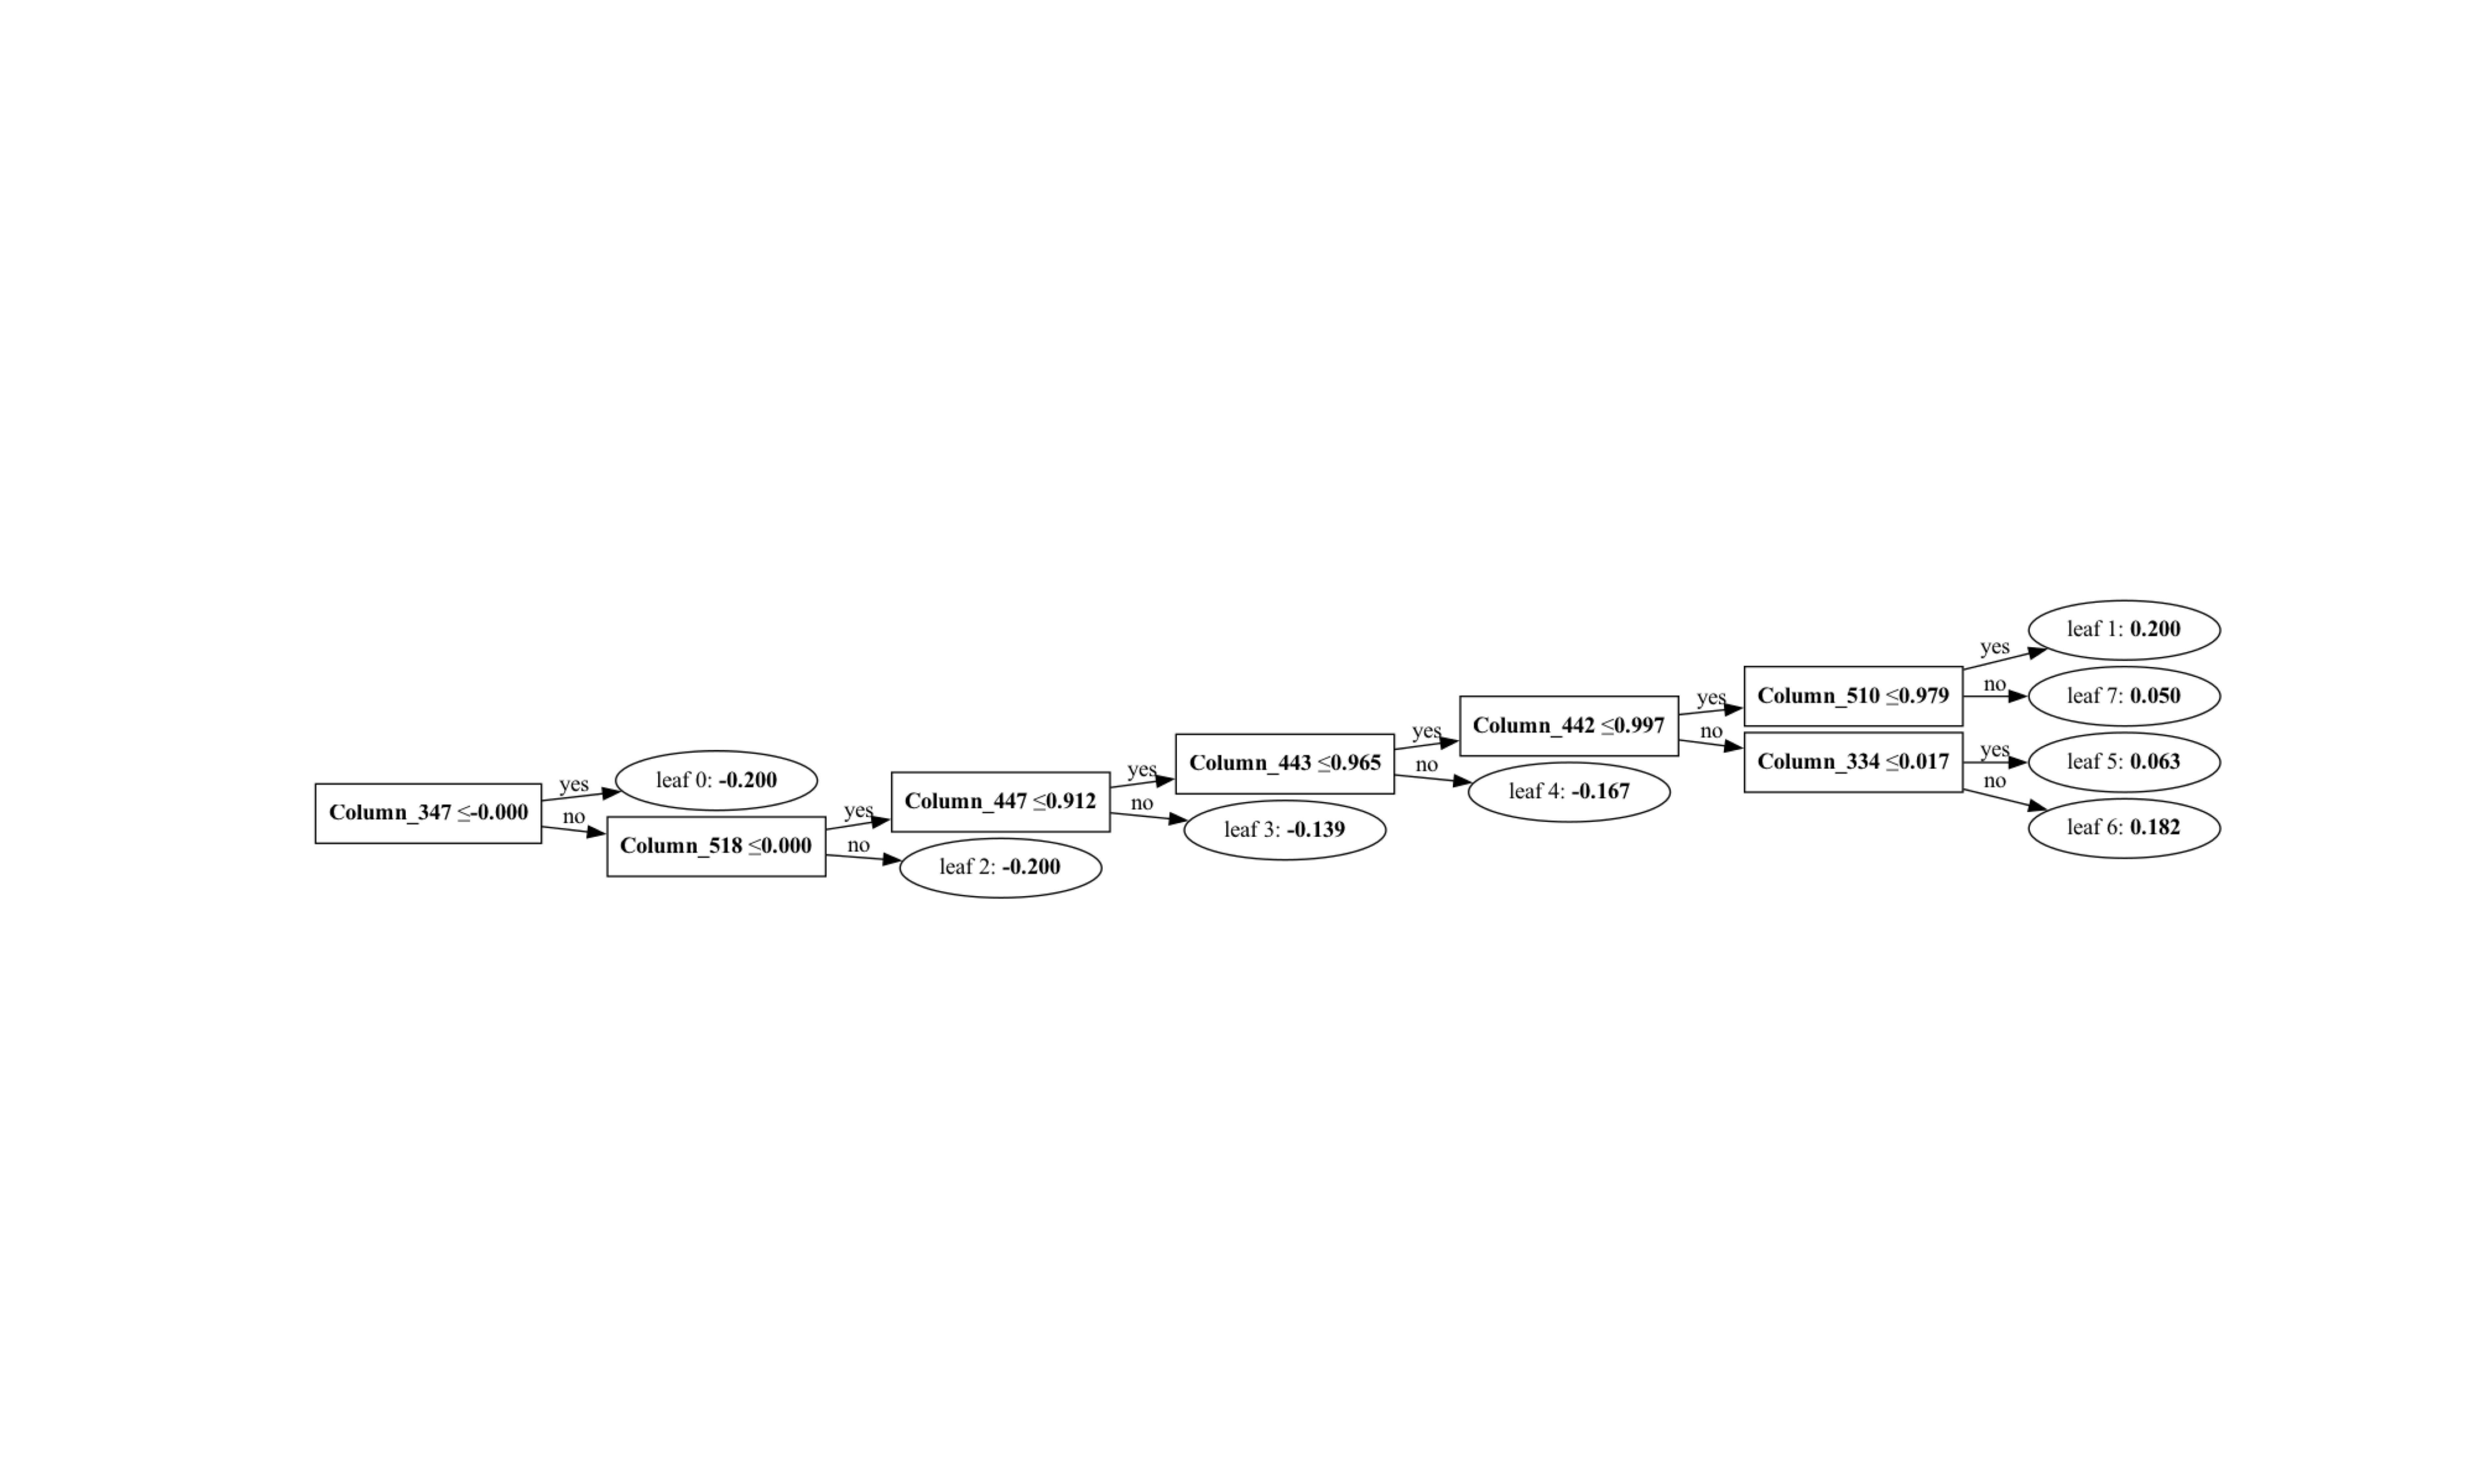
\includegraphics[width=\paperwidth, angle=270]{plots/lgbm_tree.pdf}
    \caption{LightGBM Decision Making Process. You might want to zoom in and rotate the image to see the details}
    \label{fig:catboost-decision}
\end{figure}

\subsection{Catboost Decision making process}
The best set of parameters for Catboost so far is:

\begin{table}[H]
\centering
\begin{tabular}{ll}
\textbf{Parameter} & \textbf{Value} \\
\hline
Depth & 6 \\
Iterations & 100 \\
Learning Rate & 0.1 \\
\end{tabular}
\end{table}
Thanks to the parallelization of the training process and the auto-overfit detection of the Catboost package, the training process was super fast (within 5 seconds). Here's a graph demonstrating the decision making process of catboost. The column is the index value of the feature dataset.

\newpage
\begin{figure}[H]
    \centering
    
\includegraphics[width=\paperwidth, angle=270]{plots/catboost_tree.pdf}
    \caption{Catboost Decision Making Process. You might want to zoom in and rotate the image to see the details}
    \label{fig:catboost-decision}
\end{figure}

\end{document}
